%% 
%% Copyright 2007, 2008, 2009 Elsevier Ltd
%% 
%% This file is part of the 'Elsarticle Bundle'.
%% ---------------------------------------------
%% 
%% It may be distributed under the conditions of the LaTeX Project Public
%% License, either version 1.2 of this license or (at your option) any
%% later version.  The latest version of this license is in
%%    http://www.latex-project.org/lppl.txt
%% and version 1.2 or later is part of all distributions of LaTeX
%% version 1999/12/01 or later.
%% 
%% The list of all files belonging to the 'Elsarticle Bundle' is
%% given in the file `manifest.txt'.
%% 

%% Template article for Elsevier's document class `elsarticle'
%% with numbered style bibliographic references
%% SP 2008/03/01

\documentclass[preprint,1p]{elsarticle}
\usepackage{graphicx}
\pdfoutput=1
\biboptions{numbers,sort&compress}

%% Use the option review to obtain double line spacing
%% \documentclass[authoryear,preprint,review,12pt]{elsarticle}

%% Use the options 1p,twocolumn; 3p; 3p,twocolumn; 5p; or 5p,twocolumn
%% for a journal layout:
%% \documentclass[final,1p,times]{elsarticle}
%% \documentclass[final,1p,times,twocolumn]{elsarticle}
%% \documentclass[final,3p,times]{elsarticle}
%% \documentclass[final,3p,times,twocolumn]{elsarticle}
%% \documentclass[final,5p,times]{elsarticle}
%% \documentclass[final,5p,times,twocolumn]{elsarticle}

%% For including figures, graphicx.sty has been loaded in
%% elsarticle.cls. If you prefer to use the old commands
%% please give \usepackage{epsfig}

%% The amssymb package provides various useful mathematical symbols
\usepackage{amssymb}
\usepackage{lineno}
\usepackage{hyperref}

%% The amsthm package provides extended theorem environments
%% \usepackage{amsthm}

%% The lineno packages adds line numbers. Start line numbering with
%% \begin{linenumbers}, end it with \end{linenumbers}. Or switch it on
%% for the whole article with \linenumbers.
%% \usepackage{lineno}

%% Title, authors and addresses
%% use the tnoteref command within \title for footnotes;
%% use the tnotetext command for theassociated footnote;
%% use the fnref command within \author or \address for footnotes;
%% use the fntext command for theassociated footnote;
%% use the corref command within \author for corresponding author footnotes;
%% use the cortext command for theassociated footnote;
%% use the ead command for the email address,
%% and the form \ead[url] for the home page:
%% \title{Title\tnoteref{label1}}
%% \tnotetext[label1]{}
%% \author{Name\corref{cor1}\fnref{label2}}
%% \ead{email address}
%% \ead[url]{home page}
%% \fntext[label2]{}
%% \cortext[cor1]{}
%% \address{Address\fnref{label3}}
%% \fntext[label3]{}


\journal{Nucl. Instrum. Meth. A}

\begin{document}
  
%\maketitle
%\flushbottom
\linenumbers

\begin{frontmatter}

\title{Light Based Precision Timing Detectors with SiPM Readout}

\author[1]{A.~Bornheim}
\author[2]{M.~H. Hassanshahi}
\author[1]{M.~Griffioen}
\author[1]{J.~Mao}
\author[1]{A.~Mangu}
\author[1]{C.~Pena}
\author[1]{M.~Spiropulu}
\author[1]{S.~Xie \corref{cor}}
\ead{sixie@hep.caltech.edu}
\author[1]{Z.~Zhang}
\address[1]{California Institute of Technology, Pasadena, CA, USA}
\address[2]{Institute for Research in Fundamental Science, Tehran, Iran}
\cortext[cor]{Corresponding author}


\begin{abstract}
Detectors based on scintillation light are particularly well suited for precision timing applications with 
resolutions of a few 10 ps and below. The large primary signal and the fast initial rise of the scintillation
light yield very favorable signal to noise conditions with fast signals. In this paper we describe timing 
studies with a LYSO-based sampling calorimeter with wavelengths shifting capillary light extraction and silicon
photo multipliers as sensors. We study the contributions of all steps of the signal generation to 
the final timing resolution, and demonstrate its feasibility as a radiation-hard technology for calorimeters
at high intensity hadron colliders.
\end{abstract}

\begin{keyword}
SiPM \sep Timing \sep pico second
\end{keyword}

\end{frontmatter}

%% \linenumbers
%
%% main text
%
\section{Introduction}
\label{sec:introduction}

%Scintillating materials are widely used in detectors of ionizing radiation. They
%are very common as primary sensors in calorimetric applications, either serving
%simultaneously as an absorber material, such as solid crystals, or in
%combination with passive absorbers in a layered arrangement, referred to as
%sampling calorimeters. Scintillators are also used to detect charged particles
%where they achieve a very high efficiency with a layer of thickness of about a
%few millimeters. LYSO has been proposed as a scintillating crystal for future
%calorimeters due to its large scintillation light yield~\cite{LYSOProperties,
%Yang:2015nsa}. To convert the primary scintillation light signal into an
%electrical signal a photodetector is coupled to the scintillator volume, either
%directly or via a light guiding structure. Silicon Photo Multipliers (SiPM) are
%a common choice as a photodetector in contemporary applications. In this paper
%we present studies on SiPMs and a LYSO-based sampling calorimeter with
%SiPM readout with a focus on precise timing measurements. 

Precise time of arrival measurements have recently drawn much attention in the
context of detector R\&D for the high luminosity upgrade of the Large Hadron
Collider (HL-LHC) as well as for future high energy hadron colliders. These
hadron colliders must provide large instantaneous luminosity well above
$10^{35}$~$\mathrm{cm}^{-2}\mathrm{s}^{-1}$. With accelerator and particle
detector capabilities currently under design, such a high instantaneous
luminosity will result in up to 200 simultaneous interactions (pileup) per bunch
crossing. The ability to associate the origin of particles with different
interaction points is crucial to the physics program, and precision timing would
provide a new tool for achieving it, independently from track reconstruction.


Precision timing detectors can be used to discriminate
between particles produced by different inelastic collisions \cite{adielba}. For
colliding particle beams with time spread of the order of $150$--$200$~ps, as
projected for the HL-LHC, a detector that can measure the time of arrival of
particles can identify and reject particles from pileup collisions based on
their time of arrival. Therefore with a timing detector with a timing precision
of $20$--$30$~ps, the number of pileup collisions which cannot be rejected based
on their time of arrival will be about $20$ to $40$ and is similar to
operational conditions in Run 2 of the LHC. A timing resolution in the range of
$30-50$~ps is also very interesting for optical time projection chambers which
are discussed for large volume detectors in neutrino experiments and
neutrino-less double-beta decay~\cite{Aberle:2013jba, otpc}. 

In our previous work in Ref.~\cite{Anderson:2015gha}, we demonstrated the
feasibility of achieving $30$~ps resolution for electromagnetic showers using a
sampling calorimeter based on LYSO crystal scintillators. Using micro-channel
plate photomultipliers (MCP-PMTs) to read out photons on the edge of each LYSO
layer, we achieved a time resolution of $55$~ps for electrons with $32$~GeV of
energy. Using wavelength-shifting fibers to extract the light into the MCP-PMTs,
we achieved a time resolution close to $100$~ps. We concluded that the goal of
$30$~ps time resolution was within reach provided that we can realize similar
performance using more economical photodetectors, extract the light using means
that are radiation-hard, and achieve improved light collection efficiency. In
this paper, we report on updated studies that demonstrate the time resolution
performance using silicon photomultiplier (SiPM) detectors that are more
economically scalable to the size of modern collider experiments, and 
radiation-hard wavelength-shifting quartz capillaries 
that can maintain its transparency under the harsh radiation conditions of the HL-LHC. 

The paper is organized as follows. In Sec.~\ref{sec:sipm} we give a brief
overview of the SiPM sensors in the context of our research. In
Sec.~\ref{sec:setup} we describe the experimental techniques we employ in our
precision timing measurements as well as the specific setups we used for the
studies presented in this paper. In Sec.~\ref{sec:beamtiming} we present the
results of timing measurements using SiPMs as photodetectors to read out
scintillation light from LYSO crystals exposed to electrons in the GeV energy
range. In Sec.~\ref{sec:lasertiming} we evaluate the impact of the intrinsic
timing performance of SiPM devices on the calorimeter time measurement by
measuring the time resolution for SiPMs injected with light from a fast laser.

%
%
\section{SiPM}
\label{sec:sipm}

Silicon Photomultipliers (SiPM) are pixelated photodetectors that are widely
used in contemporary high-energy physics experiments. Their compactness and form
factor make them ideal for many applications including calorimeters and charged
particle detectors. They are also widely used for positron emission tomography
(PET) detectors together with LYSO scintillating crystals for medical imaging
purposes~\cite{Vandenberghe2016}, where new studies have improved the 
timing resolution below $100$~ps~\cite{LecoqTOFPET} and 
 can yield substantial improvements in spatial resolution and imaging 
 capabilities. The size of each SiPM device typically
ranges between $1\times 1$~$\mathrm{mm}^{2}$ and $6\times 6$~$\mathrm{mm}^{2}$,
with the size of each pixel ranging between $10\mu$m to $50\mu$m. SiPMs operate
at relatively high gain between $10^{5}$ and $10^{6}$, and have single photon detection
efficiency ranging from $10\%$ to $50\%$. 
%As each pixel operates in geiger mode, it is essentially a digital
%device. More than one photon impinging on a single pixel yields the same signal
%as a single photon impinging on that pixel. Therefore as the number of photons
%approaches the total number of pixels, the SiPM experiences a slow saturation as
%the signal response slowly becomes non-linear. Total saturation occurs 
i%f the number of photons exceed the number of pixels in the device. 


SiPMs have a typical thermal dark count rate of about
$0.1$~MHz/$\mathrm{mm}^{2}$ at room temperature, which can be strongly decreased
when operated at lower temperatures. Typical operational temperatures range from
$20$ to $30$ degrees Celsius, but can be as low as $-30$ degrees Celsius. SiPMs
have been tested for the impact of radiation damage up to an equivalent neutron
rate of $2\times10^{14}$~$\mathrm{cm}^{2}$, and its performance have been shown
to be robust when operated at temperatures below $5$~degrees
Celsius.~\cite{SiPMIrradiated1,SiPMIrradiated2}. However, when operated at the
same temperature, the thermal dark count rate increases significantly with large
irradiation. The SiPMs used for our studies are Hamamatsu 
MPPC S12571-010P and S12571-015P both of 
size $1\times1\mathrm{mm}^{2}$, and S12572-15C and S12572-25C both of size 
$3\times3\mathrm{mm}^{2}$. These SiPMs are chosen to allow us to study
the impact of the size of the sensitive area and the size of individual pixels 
on the timing performance. Studies of the impact of SiPMs from alternative 
manufacturers are left for future work. Some relevant details of the SiPM parameters
are summarized in Table~\ref{tab:SiPMParameters} below.

\begin{table}[!ht]
\begin{center}
\caption{Summary of performance parameters for SiPMs used in our studies.}
\label{tab:SiPMParameters}
\begin{tabular}{|c|c|c|c|c|}
\hline
Parameter & S12571-010C & S12571-015C & S12572-15C & S12572-25C\\
\hline
Photosensitive area              & $1\times1\mathrm{mm}^{2}$ & $1\times1\mathrm{mm}^{2}$ & $3\times3\mathrm{mm}^{2}$ & $3\times3\mathrm{mm}^{2}$\\
Pixel Pitch                            & $10\mu$m                             & $15\mu$m                             & $15\mu$m                              & $25\mu$m\\
Number of Pixels                 &  10000                                    &  4489                                      & 40000                                     & 14400                       \\
Dark Count Rate                  &  $0.1$~MHz                            &  $0.1$~MHz                            & $1$~MHz                                 & $1$~MHz                  \\
Gain                                    & $1.35\times10^{5}$                  & $2.3\times10^{5}$                & $2.3\times10^{5}$                 & $5.15\times10^{5}$  \\
Terminal Capacitance          & $35$~pF                                 & $35$~pF                                  & $320$~pF                                & $320$~pF                  \\
Spectral Response Range     & $320$-$900$~nm                  & $320$-$900$~nm                  & $320$-$900$~nm                   & $320$-$900$~nm     \\
Peak Sensitivity Wavelength & $470$~nm                              & $460$~nm                              & $460$~nm                               & $450$~nm               \\         
\hline
\end{tabular}
\end{center}
\end{table}  
%
%
\section{Setup and Experimental Apparatus }
\label{sec:setup}

We performed measurements of SiPM properties in the laboratory at Caltech using
signals from a class 3R PiLas laser which produces light at a wavelength of
$407$~nm. Beam measurements were performed at the H4 beam-line of the CERN
North-Area test-beam facility, which provides secondary beams of energies
ranging between $20$~GeV and $400$~GeV. The beams are composed of a mixture of
electrons and pions. The electron fraction in the beam is typically around 75\%.

The data acquisition (DAQ) system uses a CAEN V1742 switched capacitor digitizer
based on the DRS4 chip~\cite{DRS4}, whose electronic time resolution has been
measured to be $4$~ps. Data readout for the laser-based measurements are
triggered by an external digital trigger signal, while at the H4 beamline
readout is triggered by a signal in a photomultiplier tube coupled to a
$3$~$\mathrm{cm}$~$\times$~$3$~$\mathrm{cm}$ plastic scintillator located about
one meter upstream from our detectors. A micro-channel plate photo-multiplier
(MCP-PMT) detector is used to provide a very precise reference time-stamp in
order to measure the time resolution of the SiPM signals.

\subsection{Setup for Laser-based SiPM Timing Measurements}

SiPMs are mounted on a printed circuit board (PCB) with a clipping capacitance
circuit shown in Figure~\ref{fig:Circuit}. They are mechanically attached to an
optical breadboard enclosed within a box lined with copper foil for RF
shielding. The laser is injected via a light-guide fiber mounted on an optical
holder. The laser beam is immediately split by a 50/50 beam splitter and half of
the light is directed onto the MCP-PMT while the other half of the light is
directed onto the SiPM under test. A photograph of the setup is shown in
Figure~\ref{fig:laserSetup}. The Photek-240 MCP-PMT is used as the reference
time detector whose time resolution has been measured to be below $7$~ps for
beam particles~\cite{MCPShowerMaxPaper}. To cover a large range of laser beam
intensity, neutral density (ND) filters with ND number between 0.2 and 2.4 are
placed between the beam splitter and the SiPM under test.

\begin{figure}[htbp]
\centering
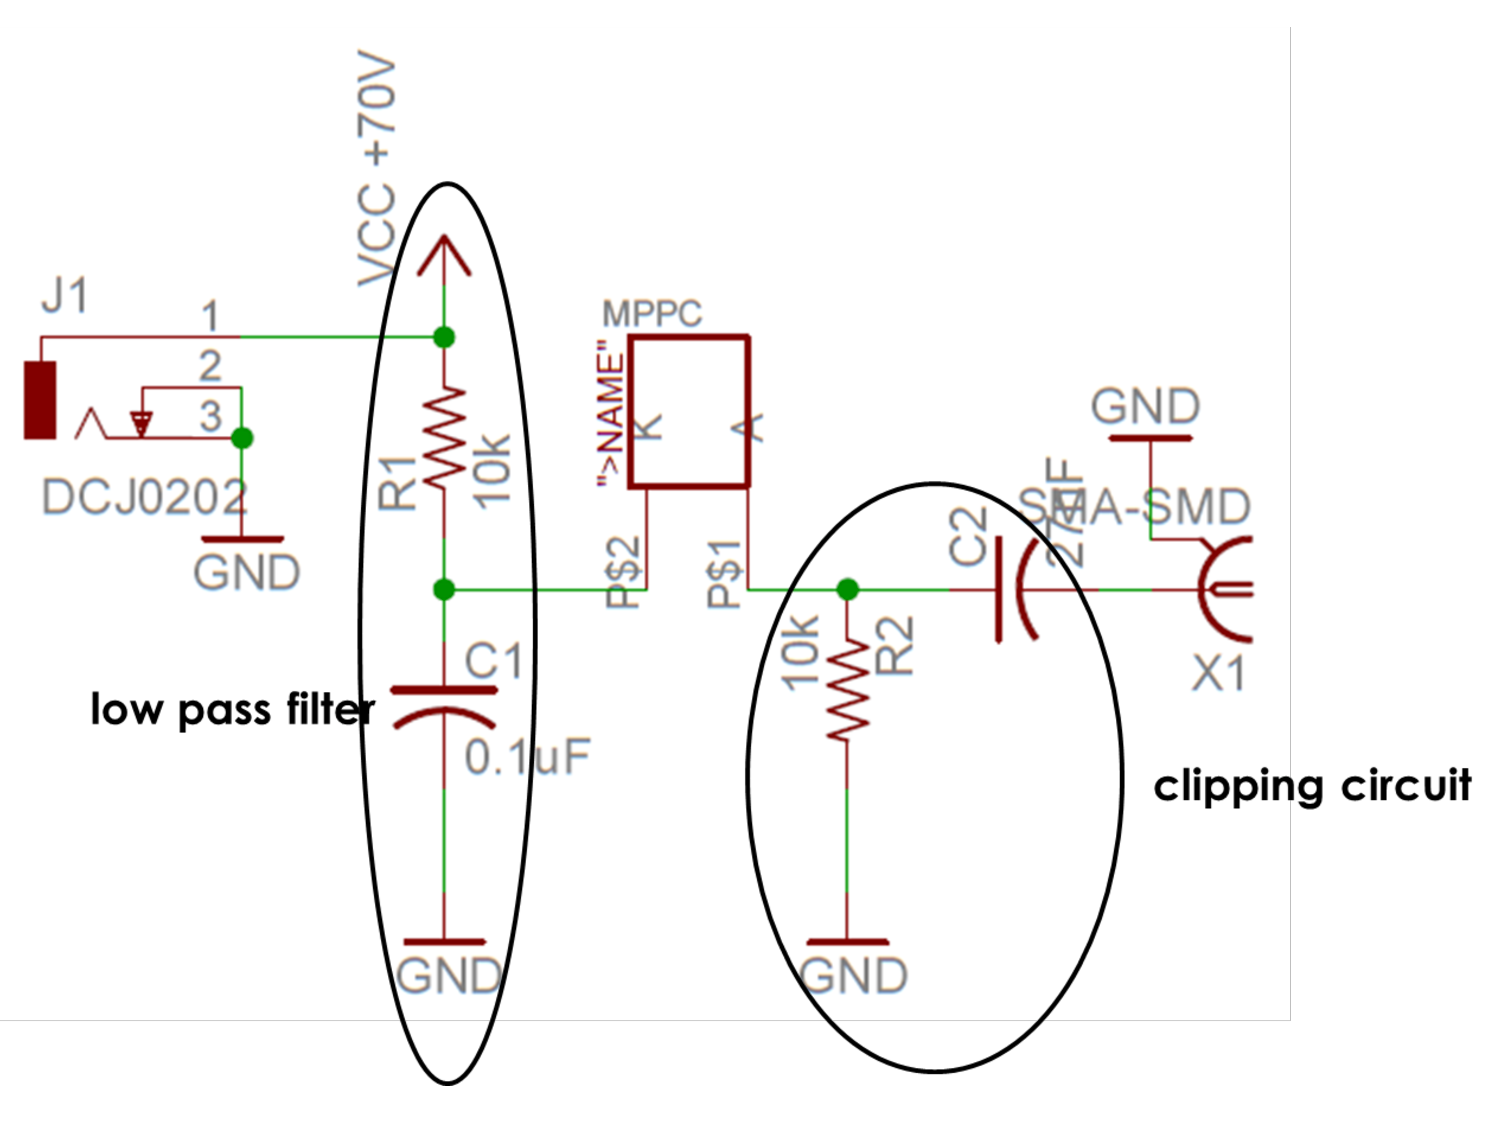
\includegraphics[width=0.60\textwidth]{figures/CircuitDiagram.pdf}
\caption{A schematic diagram of the circuit used to read out the SiPMs.}
\label{fig:Circuit}
\end{figure}



%Figure: Diagram of detector elements
\begin{figure}[htbp] 
\centering
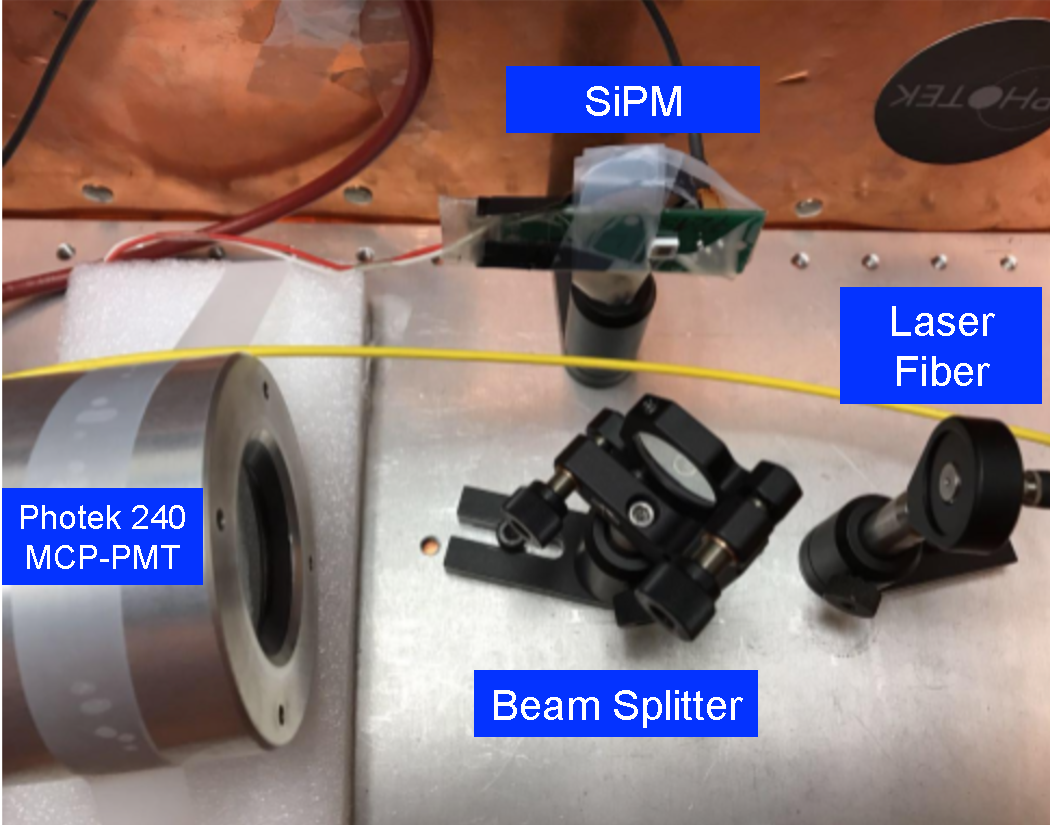
\includegraphics[width=0.80\textwidth]{figures/SiPMSetup1.pdf} 
\caption{Photograph of the Laser-based SiPM timing measurement setup.} 
\label{fig:laserSetup} 
\end{figure} 

\subsection{Setup for Timing Measurements of Scintilators with SiPM readout.}

The experimental setup we use for the calorimetric timing measurements 
is shown diagrammatically in Fig.~\ref{fig:TestbeamSchematic} and consists
of a single cell of a sampling calorimeter with 29 alternating layers of LYSO
crystal and tungsten absorber, known as a Shashlik sampling
calorimeter configuration. The lateral dimensions are
$14\times14$~$\mathrm{mm}^{2}$. The total depth of the cell is about $11.5$~cm
with the LYSO layers having a thickness of $1.5$~mm. The same cell has been used
to measure the timing performance in comparison to the timing performance of a
single monolithic crystal of LYSO~\cite{Anderson:2015gha}. A scintillator
counter of size $1\times 1$~$\mathrm{cm}^{2}$, mounted close to the calorimeter
cell, is used to select events impinging on the center of the calorimeter cell. The
scintillation light from the LYSO plates is extracted with four
wavelength-shifting (WLS) fibers. The fibers are coupled to four different types
of Hamamatsu SiPMs with 10, 15 and 25~$\mu$m pixel size and $1\times
1$~$\mathrm{mm}^{2}$ and $3\times 3$~$\mathrm{mm}^{2}$ sensor
size~\cite{hamamatsuMPPC}. The SiPMs are all read out with a DRS digitizer
through the clipping circuit shown above in Figure~\ref{fig:Circuit}. The same
clipping circuit as shown in Fig~\ref{fig:Circuit} is used for all four SiPMs.
We do not amplify the output signal of the SiPMs, only exploiting the very large
light yield of the LYSO scintillator and the intrinsic amplification of the
SiPMs. A labeled photograph of the setup in the H4 beamline is shown in
Figure~\ref{fig:TestbeamSetup}. More details of the calorimetric
performance of the Shashlik configuration are discussed in
references~\cite{shashlik1}~and~\cite{shashlik2}.

%Figure: Diagram of detector elements
\begin{figure}[htbp] 
\centering
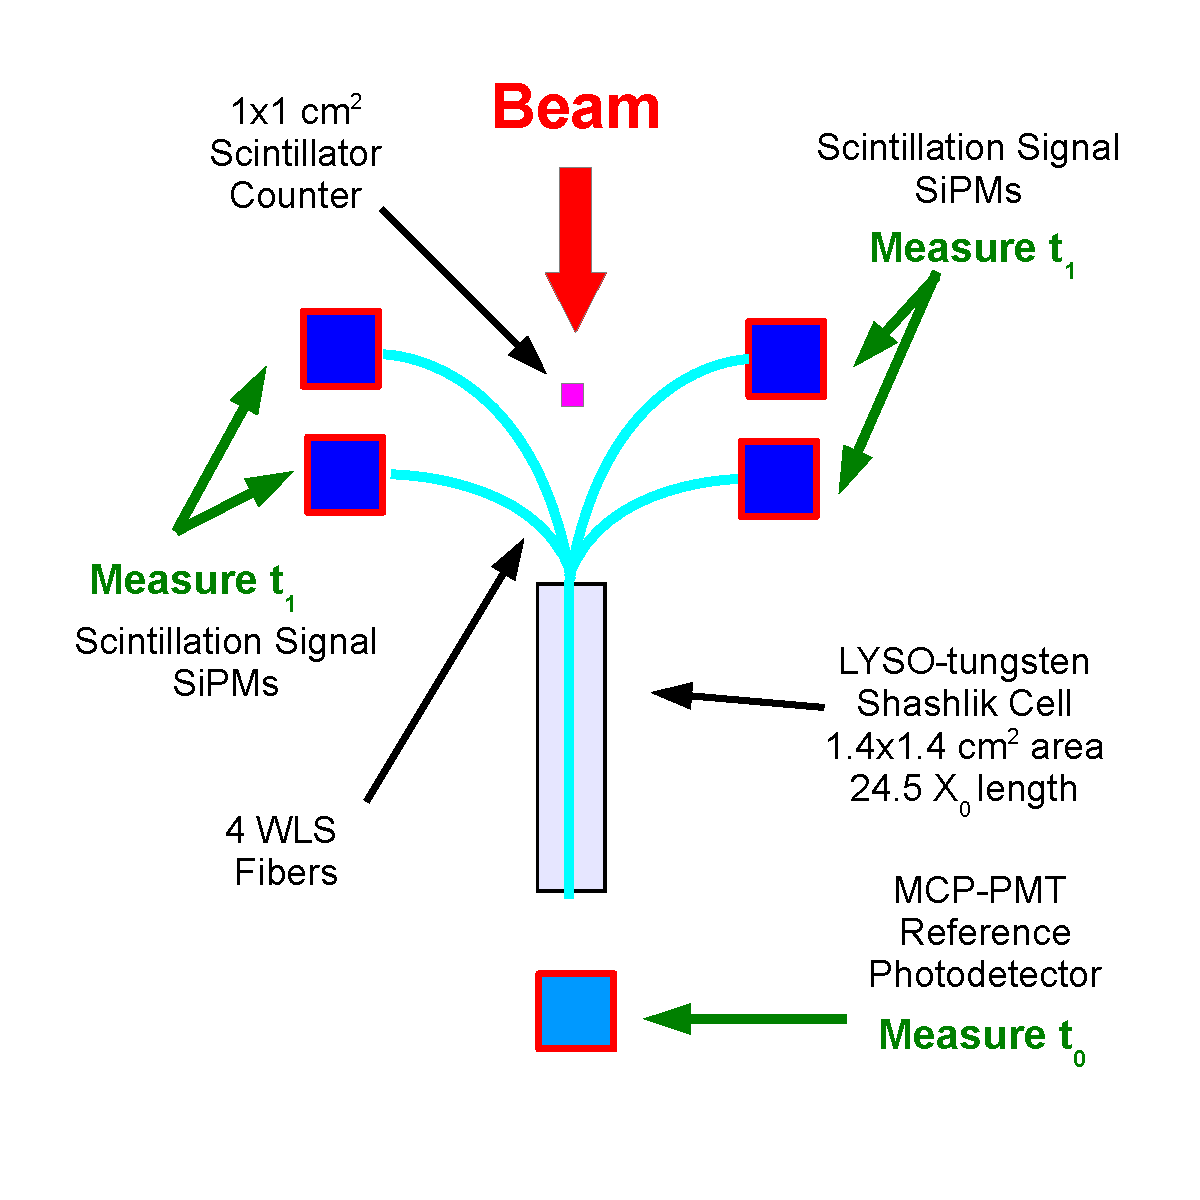
\includegraphics[width=0.80\textwidth]{figures/ShashlikFiberSetupSchematic} 
\caption{Schematic diagram of the testbeam experimental setup.} 
\label{fig:TestbeamSchematic} 
\end{figure} 

%Figure: Diagram of detector elements
\begin{figure}[htbp] 
\centering
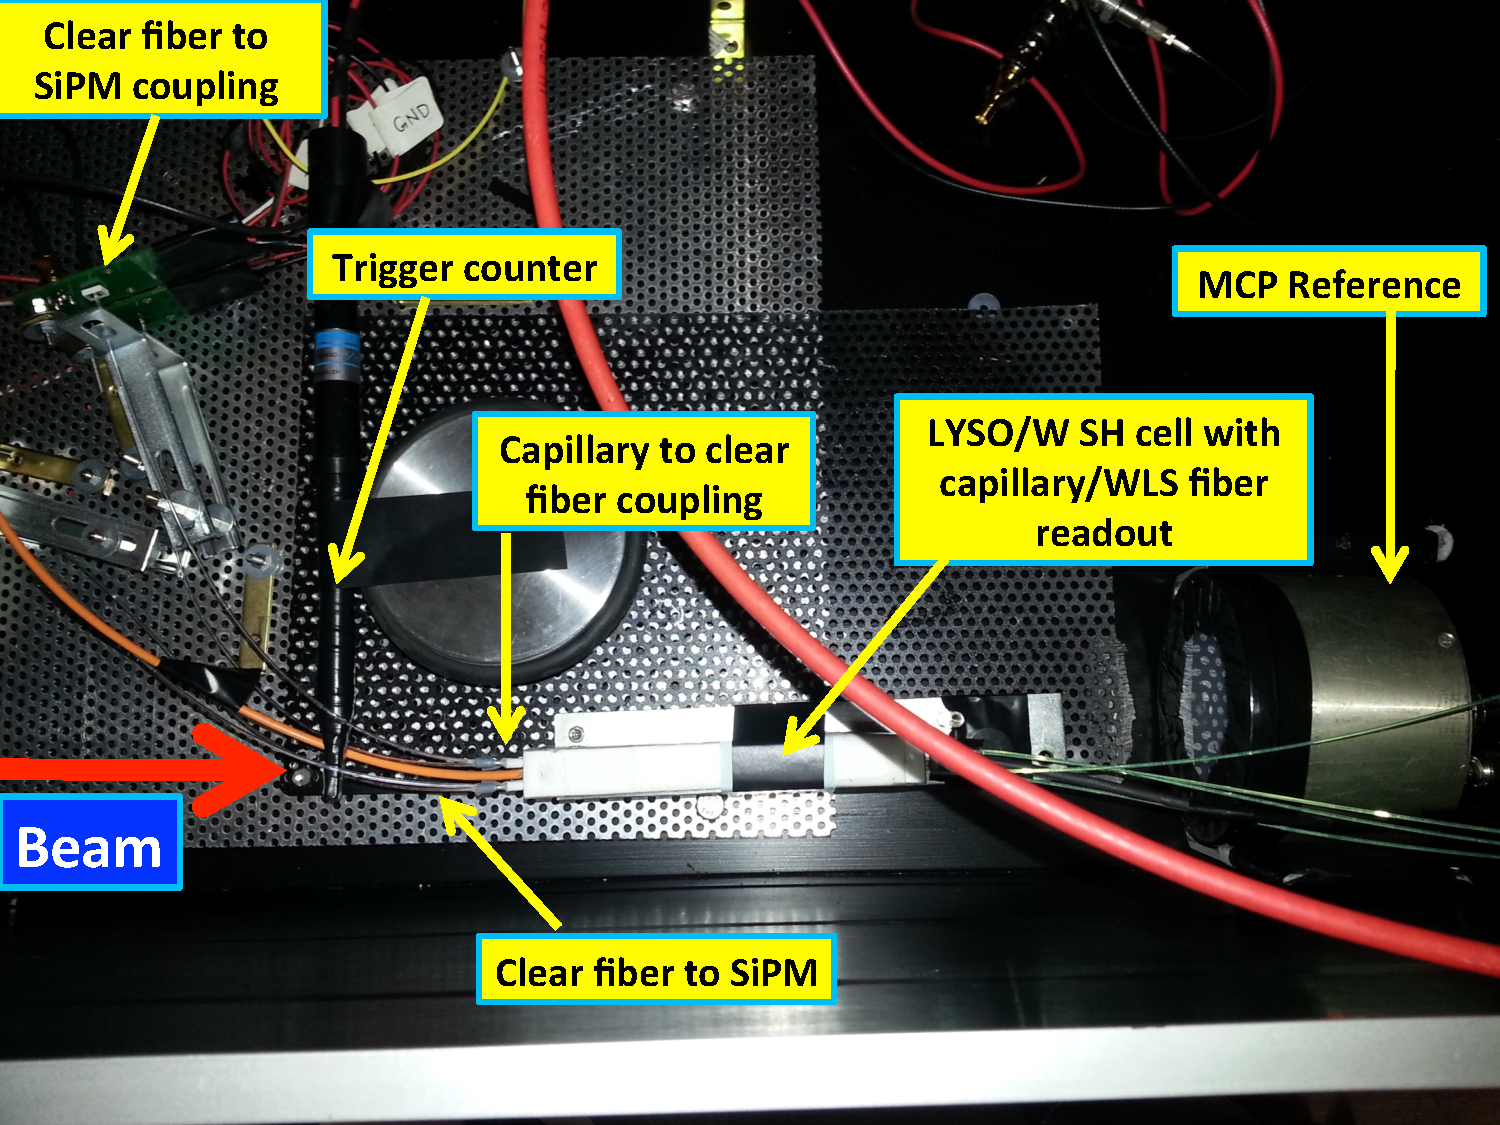
\includegraphics[width=0.95\textwidth]{figures/ShashlikTBSetupDiagram} 
\caption{Photograph of the timing measurement setup in the H4 beamline.} 
\label{fig:TestbeamSetup} 
\end{figure} 

In addition to plastic WLS fibers we also tested quartz capillaries filled with
liquid wavelength shifter using DSB as a wavelength-shifting
agent~\cite{Baumbaugh:2016vcg}. To optically couple the quartz capillaries to the
SiPMs we use a clear plastic fiber light guide which is connected to the end of
the quartz capillary with a metal sleeve tube. The same clear fiber coupler is
used for the plastic WLS fibers to maintain equivalent light collection
efficiency. The ratio of the light collection efficiency between the plastic
fibers and the quartz capillaries approximately scales with the ratio of the
diameter of the plastic fiber and the liquid core of the quartz capillary. This
ratio is about $3$ for the fibers and capillaries we used.

The Photek 240 MCP-PMT, used as the reference time detector, is placed behind the
calorimeter cell and detects secondary shower particles escaping from the
Shashlik calorimeter cell as we did in our previous studies \cite{Anderson:2015gha}.
The time resolution is extracted by measuring the time difference between the
reference counter and the calorimeter cell over an ensemble of shower events.
The time stamp for the reference counter and calorimeter cell is extracted
from a Gaussian fit to the peak and a linear fit to the rising edge, 
respectively, as described below in Section~\ref{sec:reco}.

We measure the timing performance of the calorimeter cell with high energy
electrons in a range between $20$~GeV~and~$200$~GeV in the CERN North Area
test-beam. The impact point of the electrons onto the calorimeter cell is
measured with a fiber hodoscope with a precision of better than $1$~mm. As
timing measurements are affected by shower containment, we restrict the time
measurements to events where shower containment is large. This is achieved by
using events where the beam particle impacts in the center of
the calorimeter cell within a restricted area between
$2\times2$~$\mathrm{mm}^{2}$ and $6\times8$~$\mathrm{mm}^{2}$ depending on the
exact setup. 

\subsection{Timestamp Reconstruction} \label{sec:reco} The time-stamp for all
signals is reconstructed by fitting the pulse waveform with an appropriate
functional form. Signal pulses from the MCP-PMTs as well as direct laser light
signals on the SiPMs exhibit a very fast rise and decay. Therefore, we fit a
Gaussian function to a $1.4$~ns window around the peak of the pulse and extract
the time-stamp as the mean parameter of the Gaussian function. Scintillation
signal pulses read out by the SiPM sensors have a much longer decay time. For
these signals, we fit a linear function to time sample points between $10\%$ and
$60\%$ of the pulse maximum and the time-stamp is assigned as the time at which
the fitted linear function rises to $20\%$ of the pulse maximum. More details of
the time-stamp reconstruction can be found in reference~\cite{Anderson:2015gha}.
  
%
%

\section{Timing Measurements} 

A previous study on precision timing with LYSO-based calorimeters
\cite{lysotiming} using micro-channel plate photomultipliers (MCP-PMT) 
as the primary photo-detectors achieved time resolutions at the level of 
about $100$~ps. In this paper, we present new studies of the
timing performance of LYSO-based calorimeters using silicon multi-pixel 
photon counters (SiPM). While SiPMs feature a rise time around
$1$~ns, slower than the rise time of MCPs, they allow a very good timing
performance for large, coherent signals~\cite{aashrita}. In subsection
~\ref{sec:beamtiming} we describe measurements of the timing performance 
for a LYSO-based sampling calorimeter read out by wavelength shifting 
light fibers connected to SiPMs. In subsection~\ref{sec:lasertiming}
we discuss the impact of the intrinsic timing performance of SiPMs on 
the calorimeter timing measurement studied using light signals injected
by a picosecond laser.

\subsection{Timing Performance Results from Calorimeter with SiPM Readout}
\label{sec:beamtiming}

Four different SiPMs are used to read out the four light fibers. As they each have
different gain and light collection efficiency, the signal amplitude response varies
for the four different channels. In Figure~\ref{TimeResolution} we show the time 
resolution of the four individual fibers as a function of their respective signal 
amplitudes. We observe that the time resolution improves as the amplitude of the pulses 
increases. The best time resolution per fibre is around $60$~ps for all of the channels, 
but the amplitude at which this performance is achieved varies.
Another important observation is that the time resolution measured from
the DSB-doped WLS fibers fall on the same curve as the time resolution measured from
the quartz capillaries. We conclude that the method of light extraction
impacts the time resolution only through its effect on the signal amplitude, and
no additional time jitter is introduced. 


\begin{figure}[htb]
\centering
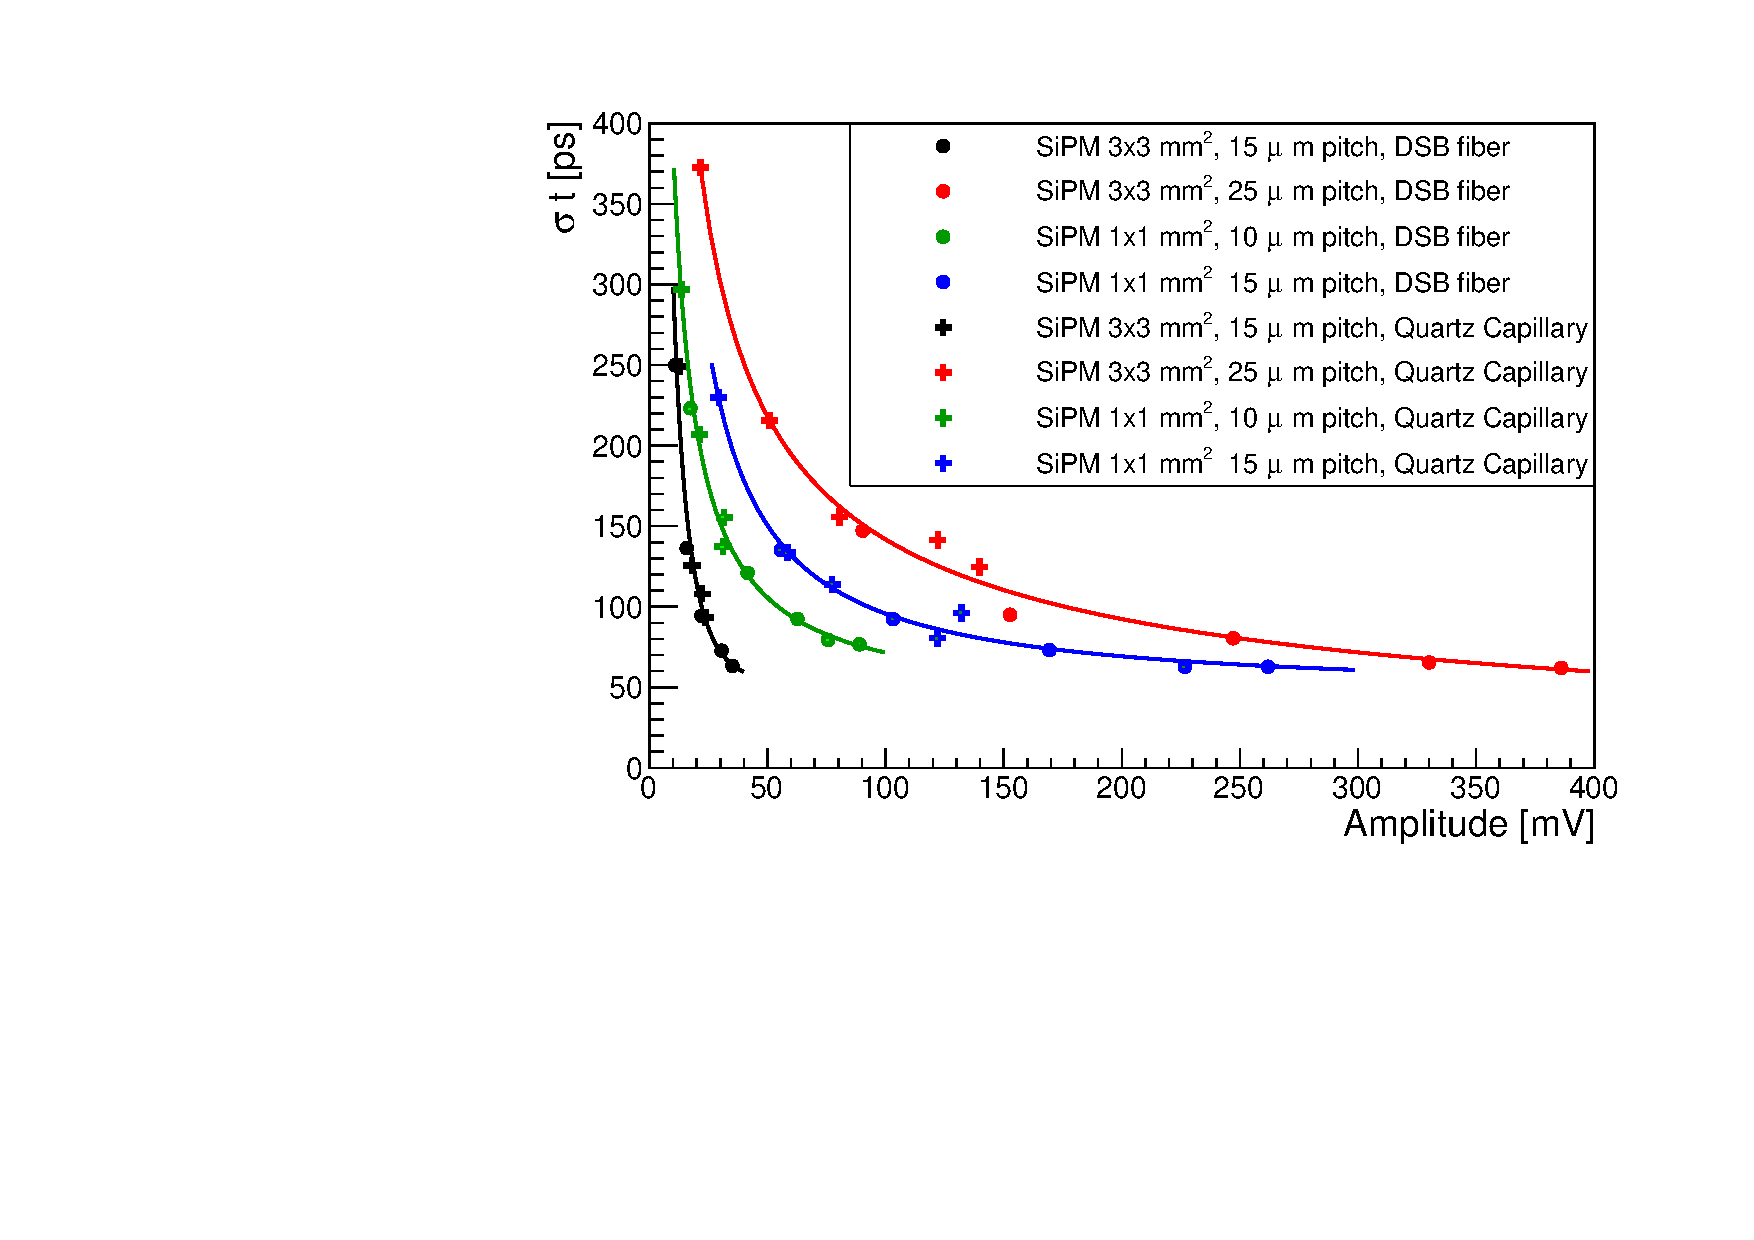
\includegraphics[width=0.99\textwidth]{figures/ShashlikTimeResolution.pdf}
\caption{\label{TimeResolution} Time resolution achieved with the calorimeter cell using the signal of each 
of the  SiPMs individually. The data for each SiPM consists of two sets, one with the DSB WLS plastic fiber shown as 
dots and one with the capillaries with a liquid DSB based WLS shown as squares. }
\end{figure}



As the time measurement precision depends on the rise time of the pulse we also
measure the time resolution as a function of the rise time for signals observed 
in the calorimeter cell shown in Figure~\ref{RiseTime}. The risetime of these signals 
are driven by the time constants of the wave length shifter as 
demonstrated in reference~\cite{Anderson:2015gha}. We observe that the risetime
ranges between $1.4$~ns and $6$~ns and that the time resolution improves 
roughly proportional to the risetime of the signals. 


\begin{figure}[htb]
\centering
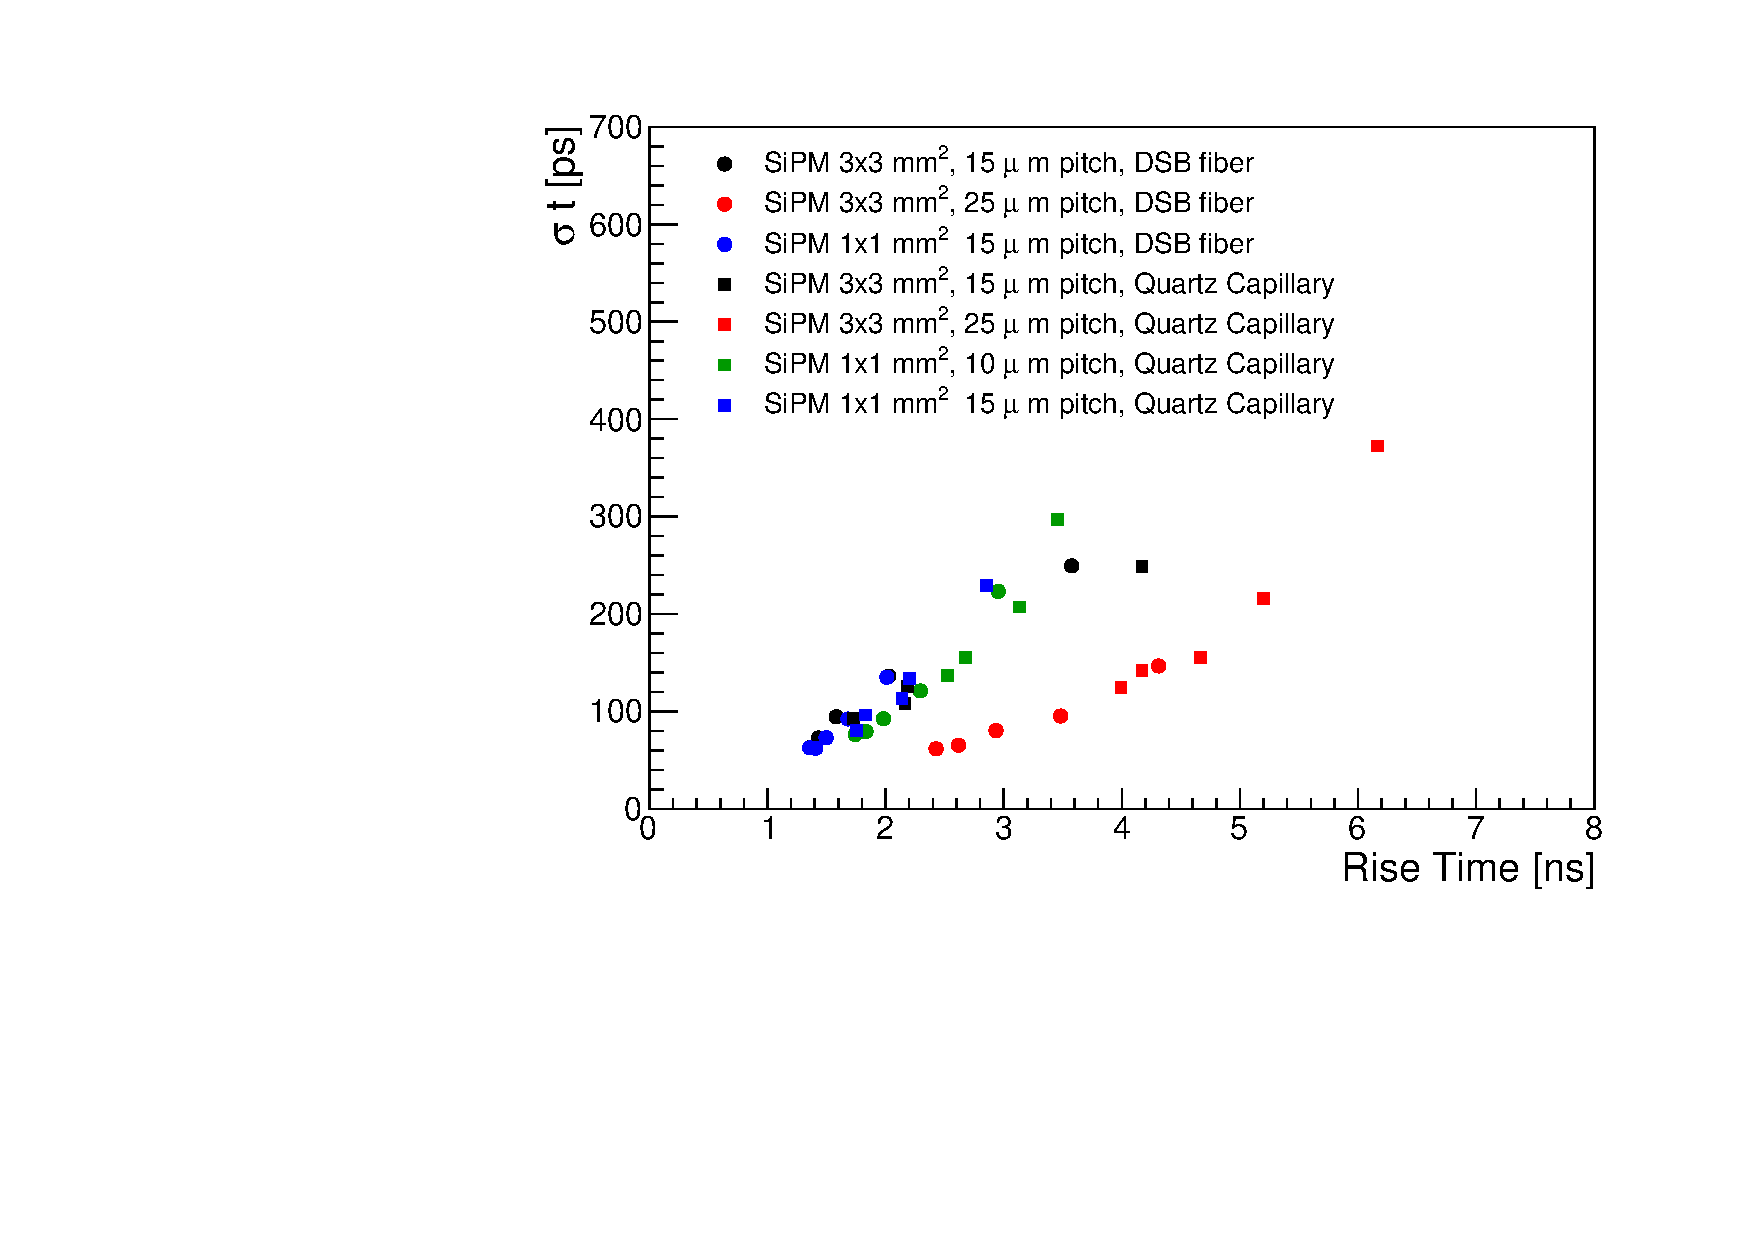
\includegraphics[width=0.99\textwidth]{figures/ShashlikTimeResolutionVsRiseTime.pdf}
\caption{\label{RiseTime}Time resolution is measured as a function of the risetime
for the four different SiPMs. The data recorded with the DSB WLS fibers and the
quartz capillaries are distinguished as dots and squares. }
\end{figure}



We show the time resolution measured as a function of the beam energy for
data read out by DSB WLS fibers and quartz capillaries in 
Figure~\ref{TimeResolutionVsEnergy}. Finally, by combining the measured timestamp
from all four SiPM channels, we can significantly improve the time resolution.
The combined time resolution measurements for the DSB WLS fibers and the quartz capillaries are shown in
Fig~\ref{TimeResolutionCombined} and demonstrate that we can achieve time resolution
below $50$~ps for high energy electromagnetic showers.


\begin{figure}[htb]
\centering
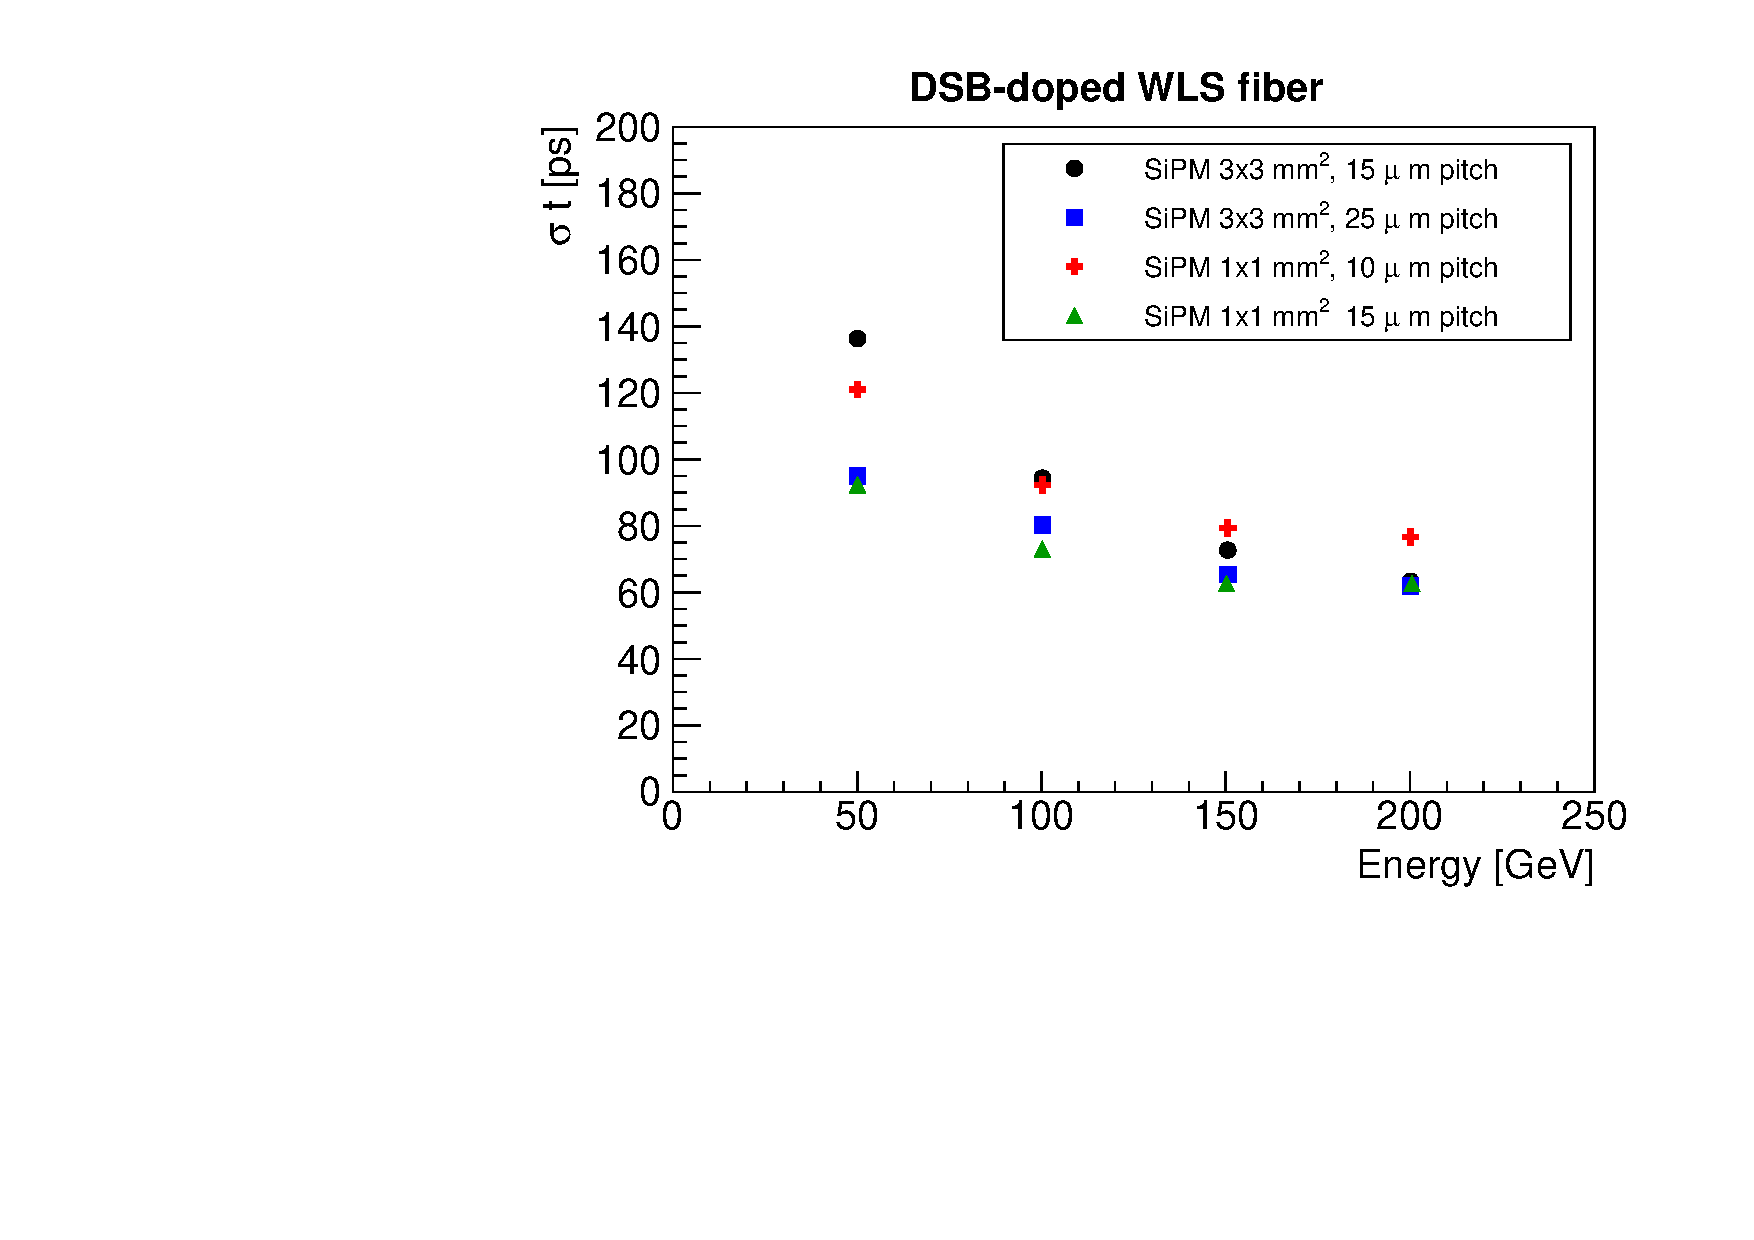
\includegraphics[width=0.49\textwidth]{figures/ShashlikTimeResolutionVsEnergy_DSB.pdf}
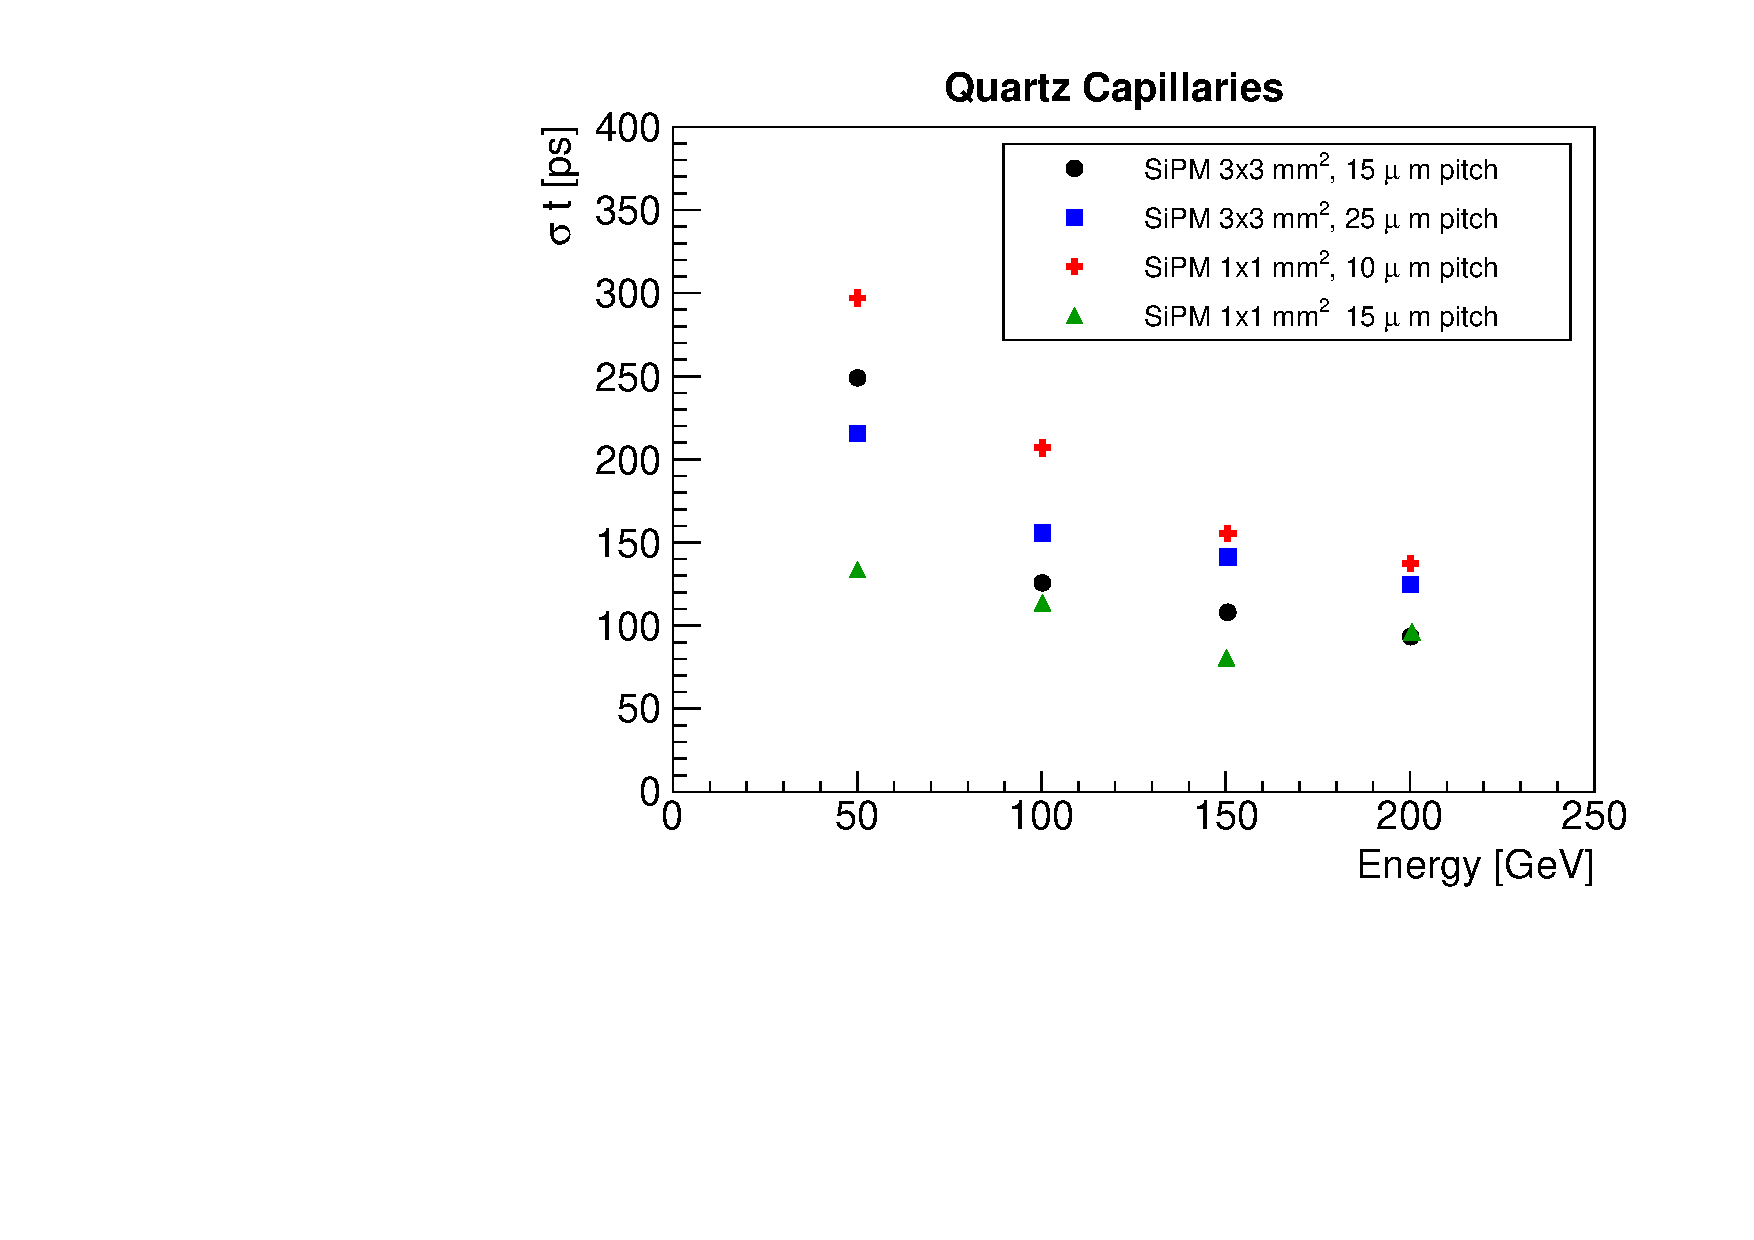
\includegraphics[width=0.49\textwidth]{figures/ShashlikTimeResolutionVsEnergy_Capillaries.pdf}
\caption{\label{TimeResolutionVsEnergy} Time resolution measured in the sampling calorimeter 
cell using the signal of each of the SiPMs individually as a function of the beam energy. 
The data taken using DSB WLS fibers are shown on
the left and the data taken using quartz capillaries are shown on the right}
\end{figure}



\begin{figure}[htb]
\centering
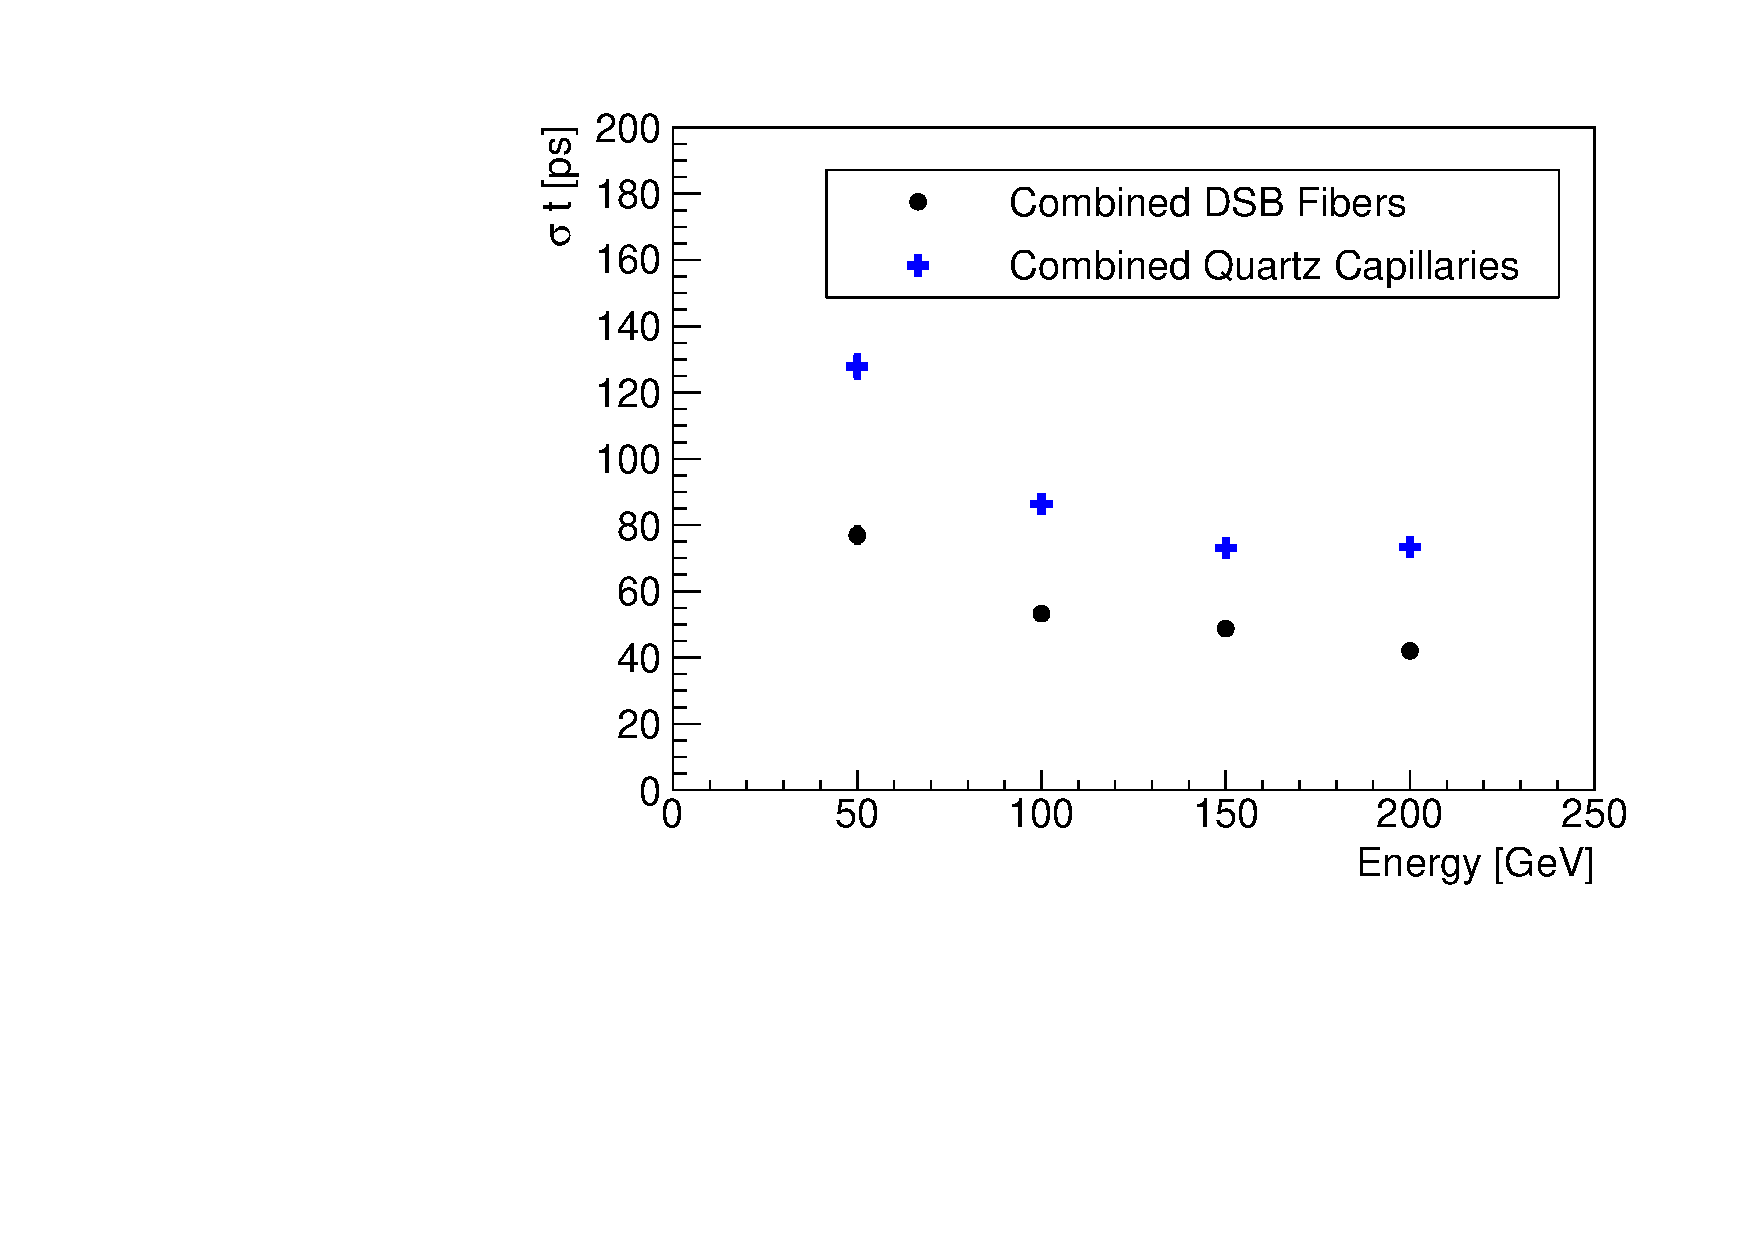
\includegraphics[width=0.8\textwidth]{figures/ShashlikTimeResolutionCombinedChannelVsEnergy.pdf}
\caption{\label{TimeResolutionCombined}  Time resolution measured in the sampling calorimeter cell combining signals from all four  
SiPMs is shown as a function of the beam energy.  The data recorded with the DSB WLS fibers and the
quartz capillaries are distinguished as dots and squares.}
\end{figure}



The light extraction efficiency of capillaries with liquid WLS remains
sufficiently high for dose rates of $100$~Mrad and beyond and for fluences of
$10^{14}$~protons/$\mathrm{cm}^{2}$ and beyond~\cite{shashlik2}. This result
demonstrates the feasibility of achieving good time resolution using a sampling
calorimeter based on LYSO which can survive in dense hadronic collision environments.
The energy resolution performance of the LYSO-tungsten cell is not limited by
photo-statistics but is rather limited by the sampling fraction. Therefore, the timing
performance could be improved by increasing the signal size, for example by 
using larger diameter capillaries.\\ 

  
%
%
\subsection{Timing Performance Results for Laser Pulses}
\label{sec:lasertiming}

To evaluate the impact of the intrinsic timing performance of the SiPMs
on the time resolution measured for the sampling calorimeter signals, 
we performed laser-based measurements for two types of SiPMs: a Hamamatsu
S12571-015P Multi-Pixel Photon Counter (MPPC) with an area of $1\times
1$~$\mathrm{mm}^{2}$ and pixel pitch size of $15$~$\mu$m, and a Hamamatsu
S12572-25C MPPC with an area of $3\times 3$~$\mathrm{mm}^{2}$ and pixel pitch
size of $25$~$\mu$m. Examples of the digitized waveforms for signals from both
SiPMs are shown in Figure~\ref{fig:pulses}.

\begin{figure}[htbp] 
\centering
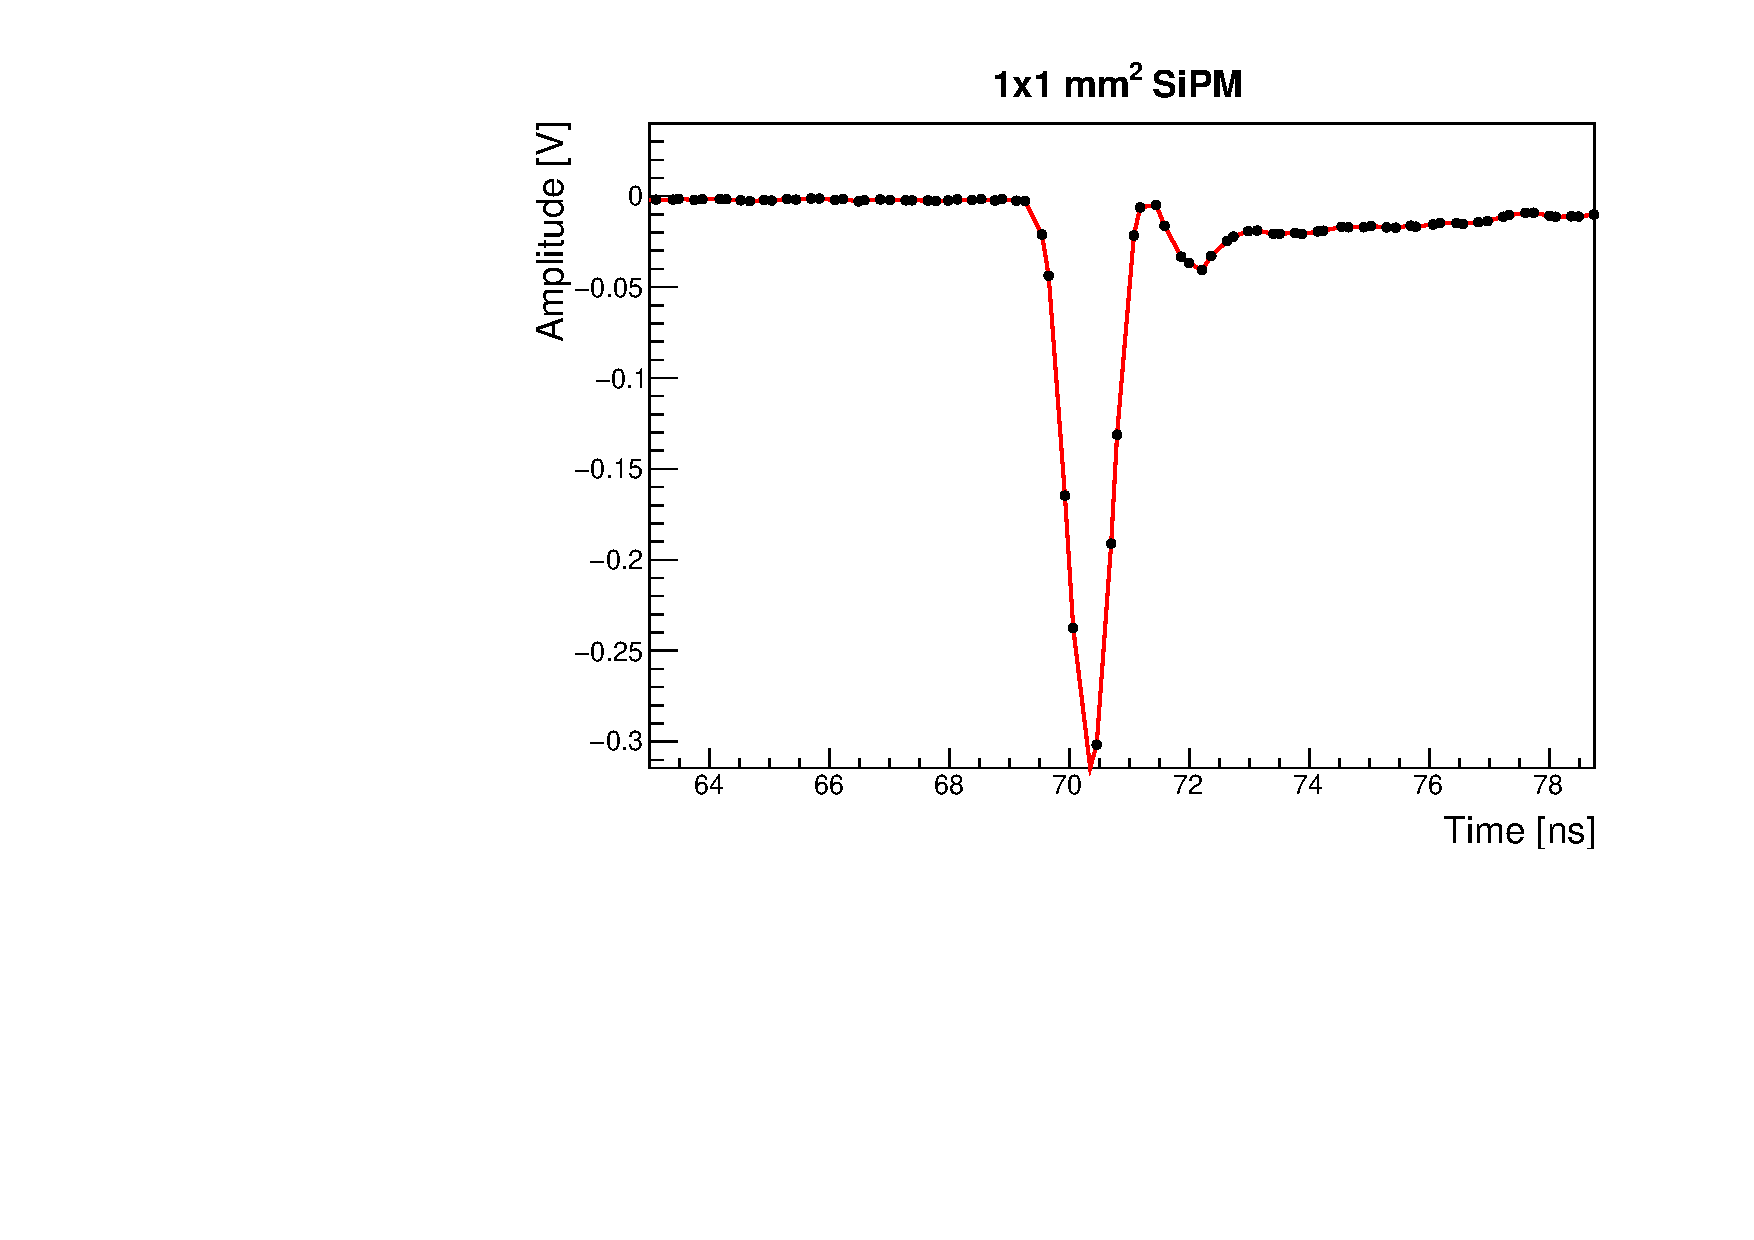
\includegraphics[width=0.49\textwidth]{figures/PulseShapeExample_1x1SiPM.pdf} 
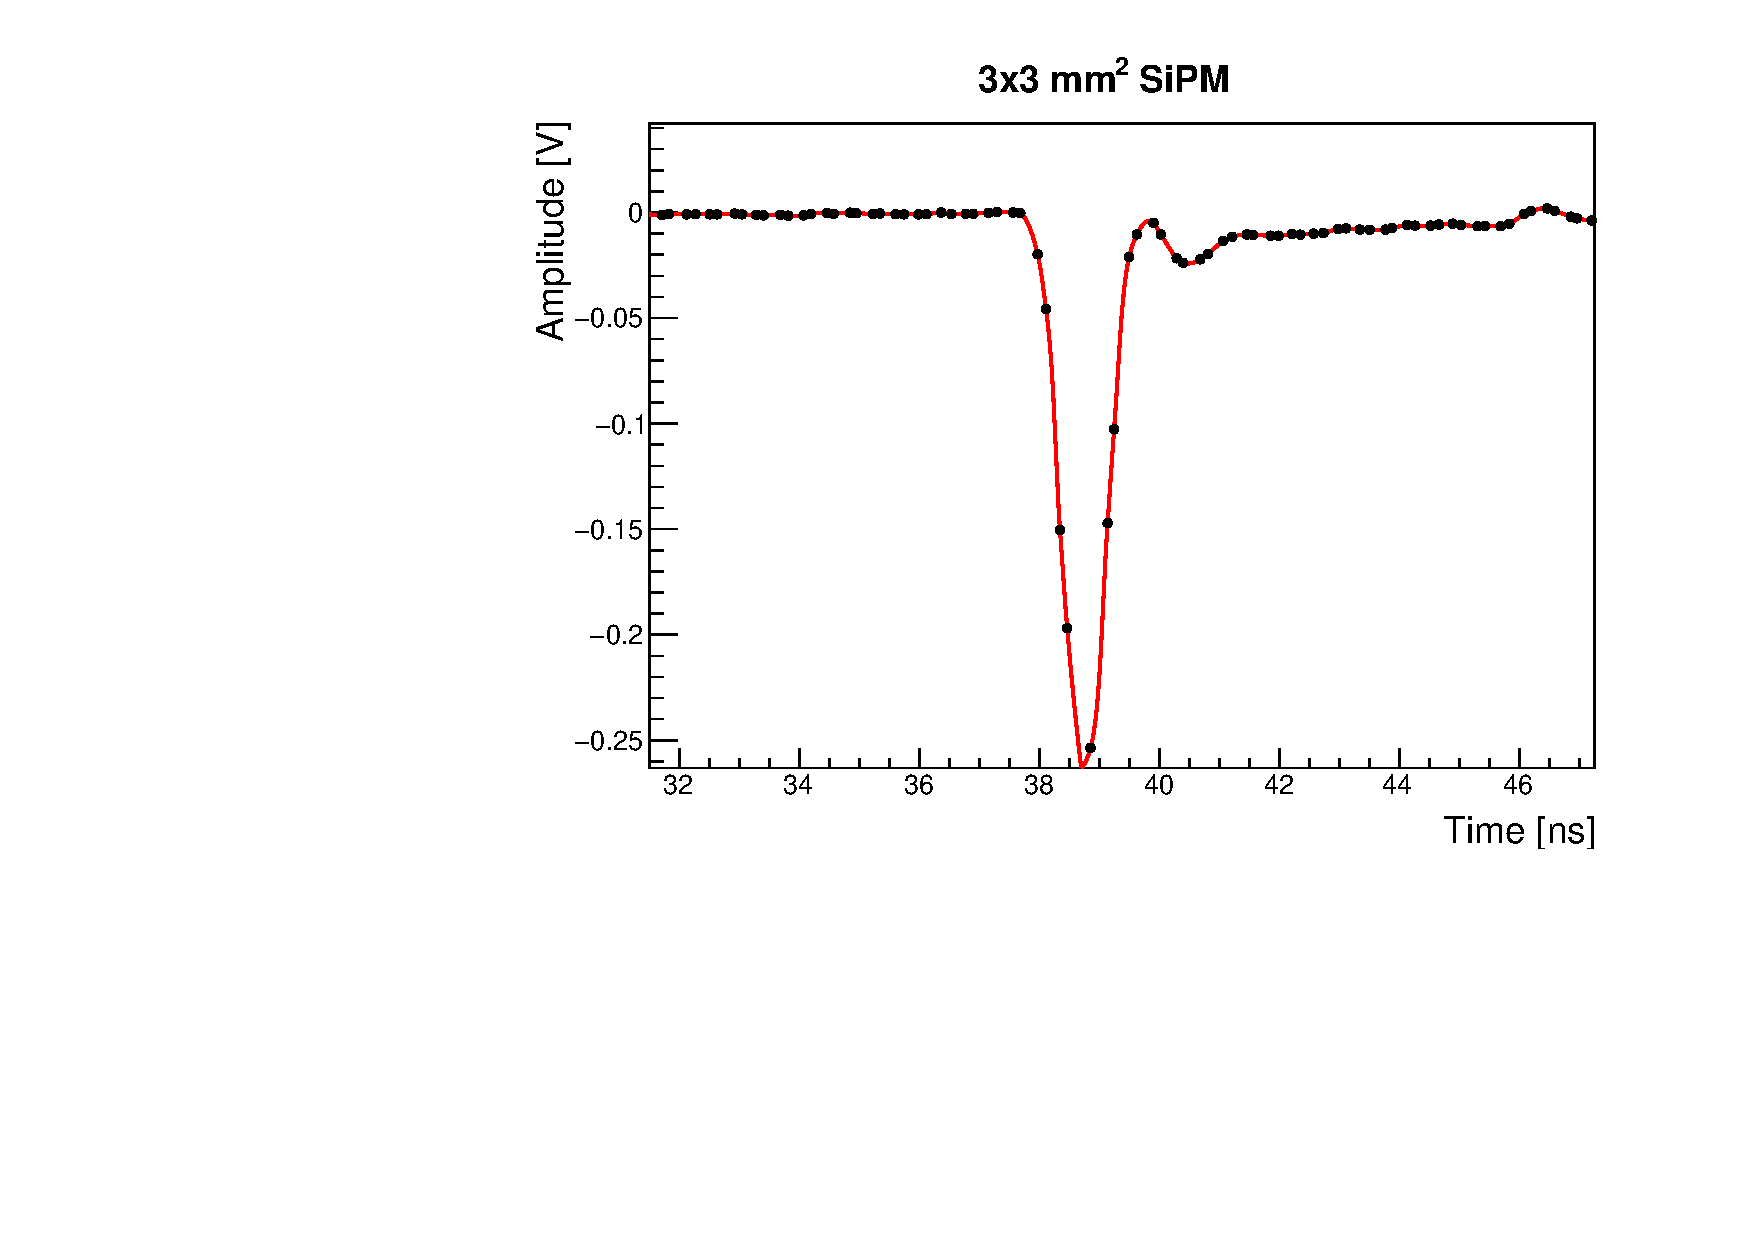
\includegraphics[width=0.49\textwidth]{figures/PulseShapeExample_3x3SiPM.pdf} 
\caption{Digitized waveforms of the signals from the PiLas laser 
in the S12571-015P and S12572-25C SiPMs.} 
\label{fig:pulses} 
\end{figure} 

Using several different neutral density (ND) filters we controlled the intensity of the photon 
beam impinging upon the SiPMs under test and achieved a large dynamic range 
of signal sizes ranging from a single incident photon to a few hundred. In 
Figure~\ref{fig:NPhotonPeaks}, we show the integrated charge distribution
for two example scenarios from which we can clearly distinguish different peaks
corresponding to different number of photoelectrons detected by the SiPMs.

\begin{figure}[htbp] 
\centering
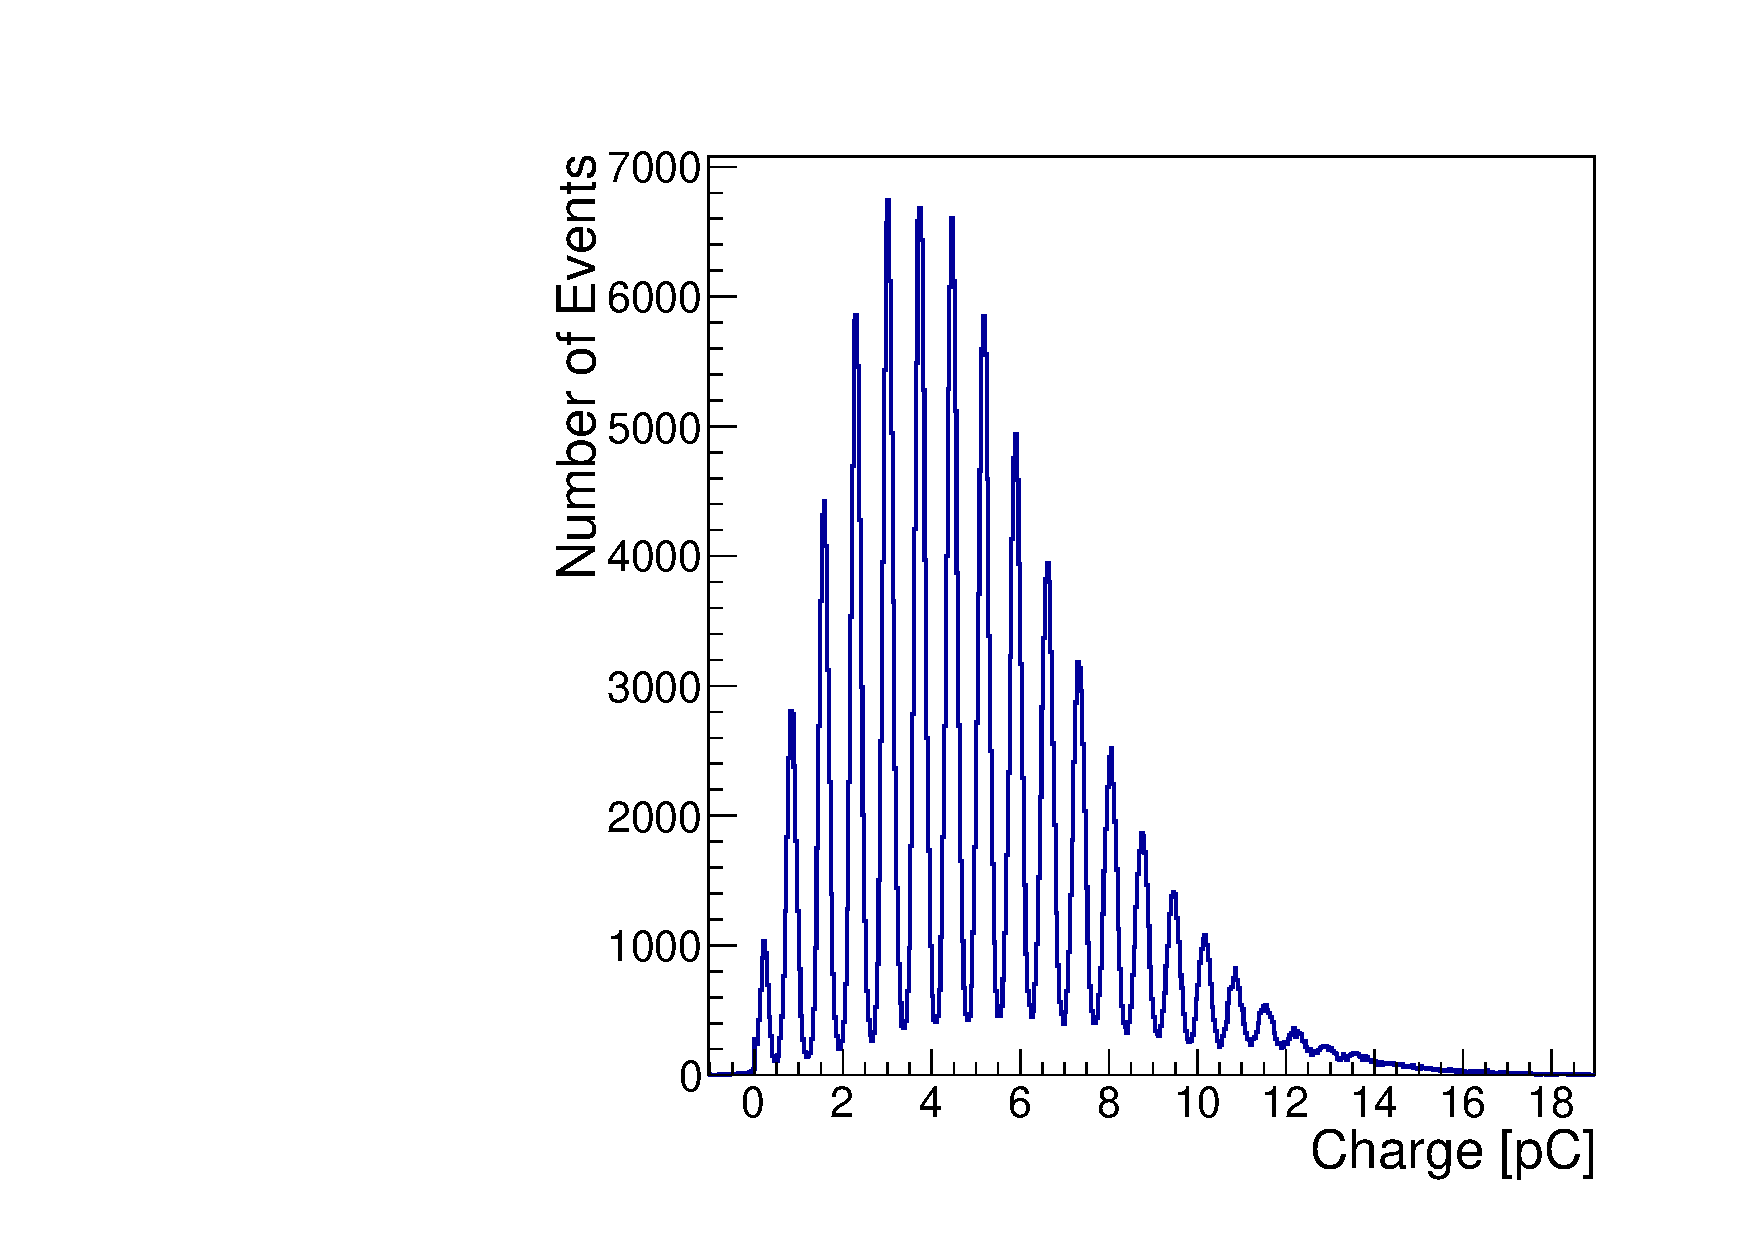
\includegraphics[width=0.49\textwidth]{figures/NPhotons1.pdf} 
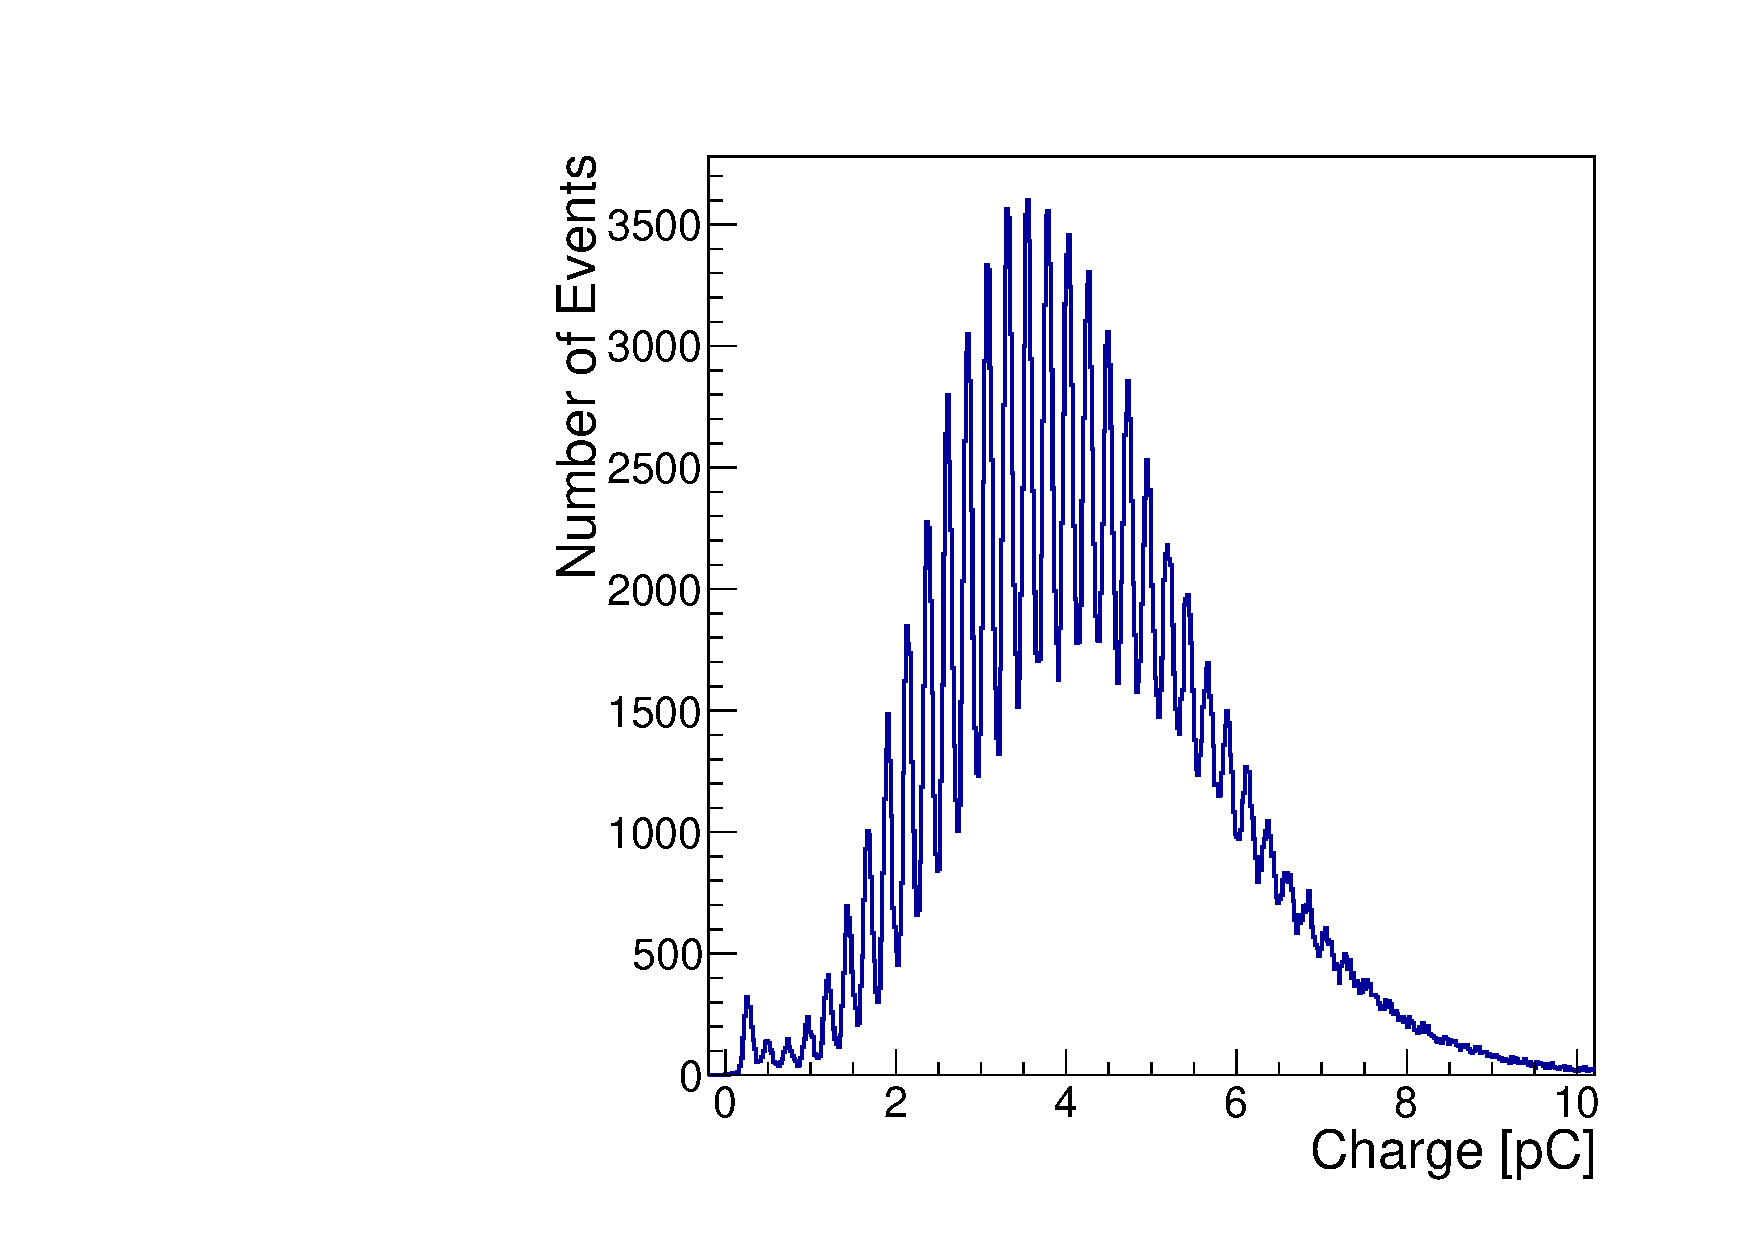
\includegraphics[width=0.49\textwidth]{figures/NPhotons2.pdf} 
\caption{The distribution of integrated charge from the SiPM sensor for data 
taken with an ND filter of 1.8 (left), and an ND filter of 1.4 (right). 
A $10$~db attenuator has been used for the plot on the right. The peaks corresponding
to different discrete numbers of photoelectrons detected by the SiPM is clearly
evident.} 
\label{fig:NPhotonPeaks} 
\end{figure} 

Using this setup, we measure the timestamps reconstructed from the SiPM signals
with respect to the reference MCP-PMT timestamp over an ensemble of events
triggered by the external laser trigger. The sigma parameter of a gaussian fit
to this distribution is taken as the time resolution measurement.
As the number of photons impinging on the SiPM can be clearly distinguished 
based on the amplitude or charge collected, we can study the dependence of the 
time resolution on the number of photons. These measurements are shown in 
Figure~\ref{fig:TimeResolutionVsNPhotons}. The amplitude for a single
photoelectron signal is estimated to be $0.6$~mV for the $1\times1$~$\mathrm{mm}^{2}$ 
S12571-015P SiPM and $0.02$~mV for 
the $3\times 3$~$\mathrm{mm}^{2}$ S12572-25C SiPM. Using these 
measurements, we can compare the time resolution of laser light signals on
SiPMs from Figure~\ref{fig:TimeResolutionVsNPhotons} to the time resolution
of electromagnetic shower signals from the WLS fiber in Figure~\ref{TimeResolution}
and conclude that the impact of the intrinsic timing performance of 
SiPM devices are small and more than a factor of $5$ smaller. Therefore the time resolution
of the calorimeter is dominated by the impact of the wavelength shifter
and the increased risetime.



\begin{figure}[htbp] 
\centering
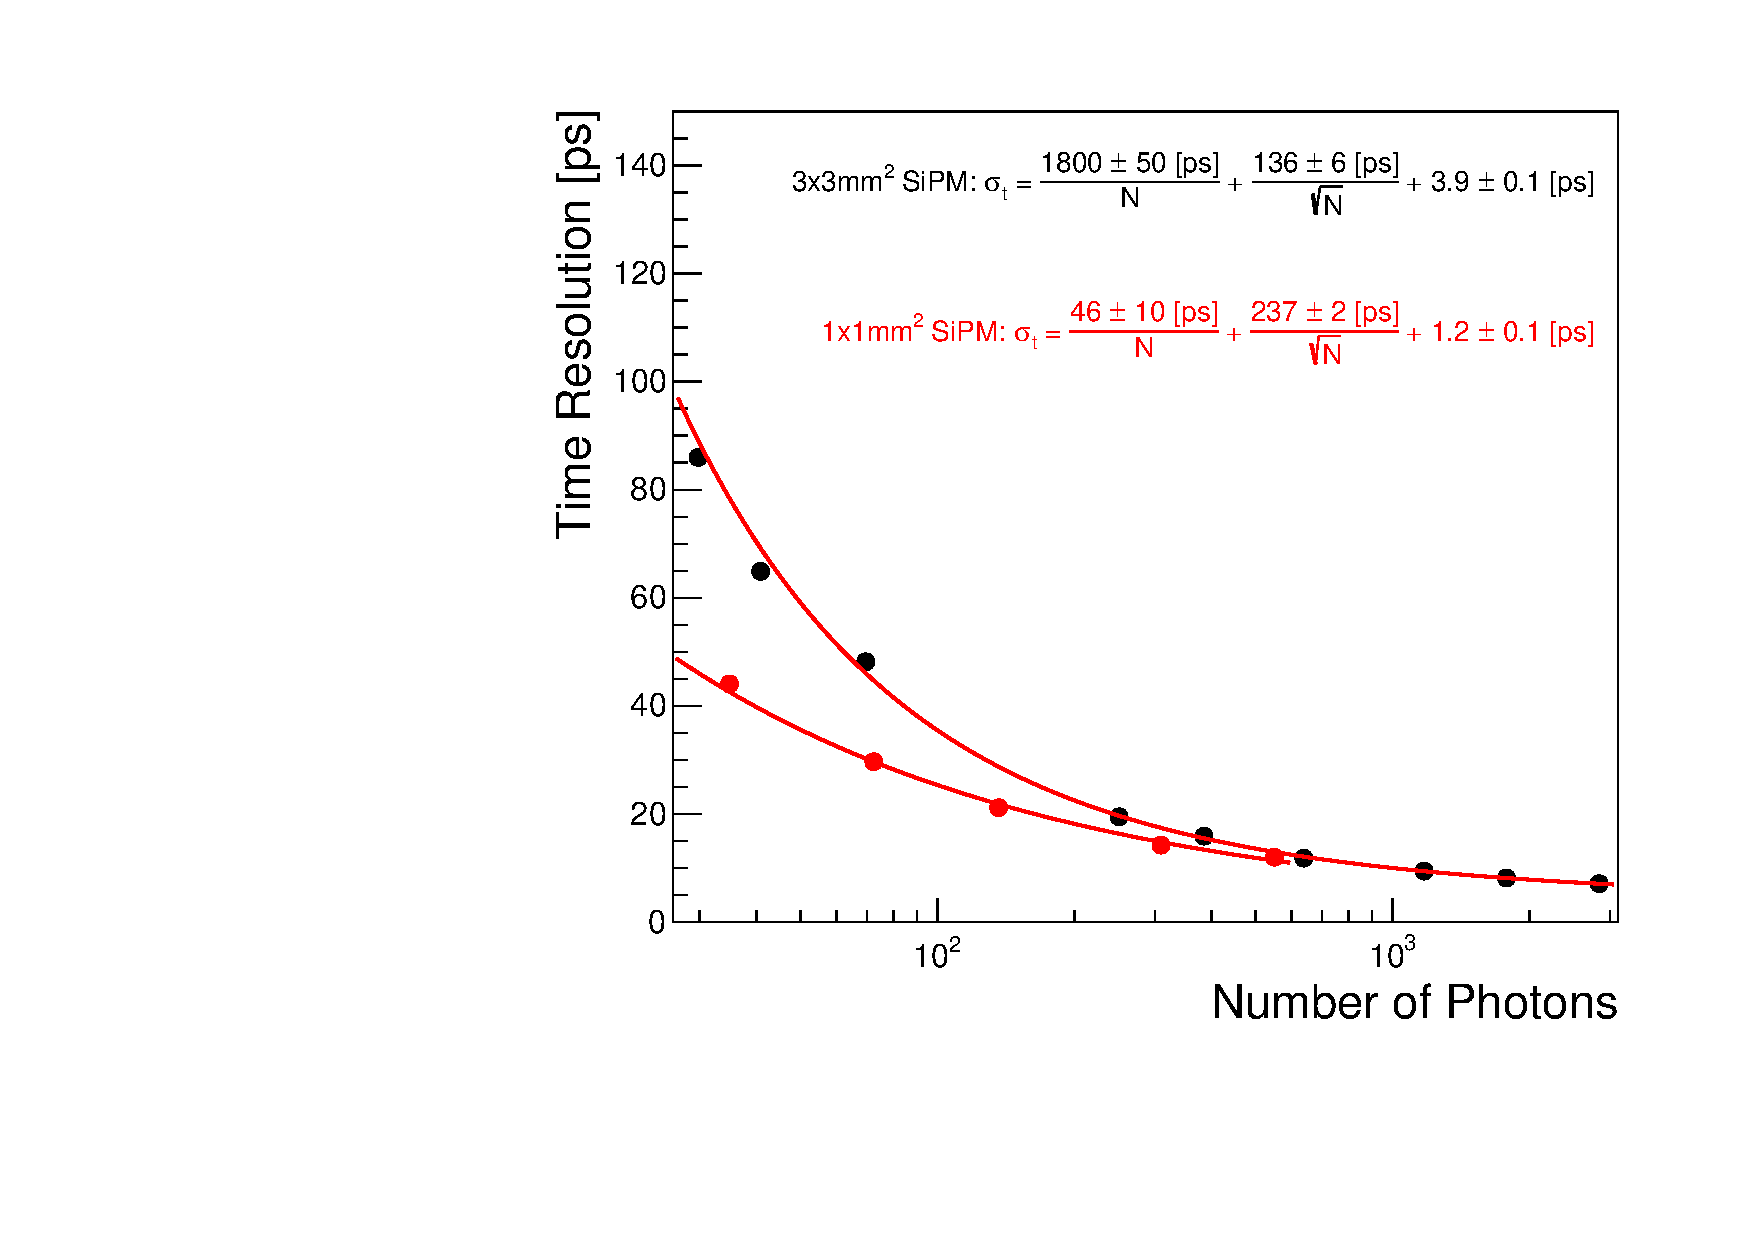
\includegraphics[width=0.49\textwidth]{figures/TimeResolutionVsNPhotons.pdf}
\caption{ The time resolution is measured as a function of the number of photons 
impinging on the SiPMs under test. The black points show measurements using the
$3\times3$~$\mathrm{mm}^{2}$ SiPM, and the red points show measurements
using the $1\times1$~$\mathrm{mm}^{2}$ SiPM. \label{fig:TimeResolutionVsNPhotons}
} 
\label{fig:pulses} 
\end{figure} 


Finally, by removing all ND filters and increasing the laser output intensity to near 
maximum, we can measure the time resolution for a very large number of photons 
to probe for the ultimate time resolution that one could achieve with a near 
infinitely large signal. In Figure~\ref{fig:LargeLightTimeResolution} we show 
the SiPM time distributions for such a scenario, and observe that the resolution 
is $12$~ps for the $1\times1$~$\mathrm{mm}^{2}$  S12571-015P SiPM and
$7$~ps for the $3\times 3$~$\mathrm{mm}^{2}$ S12572-25C SiPM. 
The measurement is also impacted by the limitation
of the digitizer electronics as its impact on the time resolution is $4$~ps. 

\begin{figure}[htbp] 
\centering
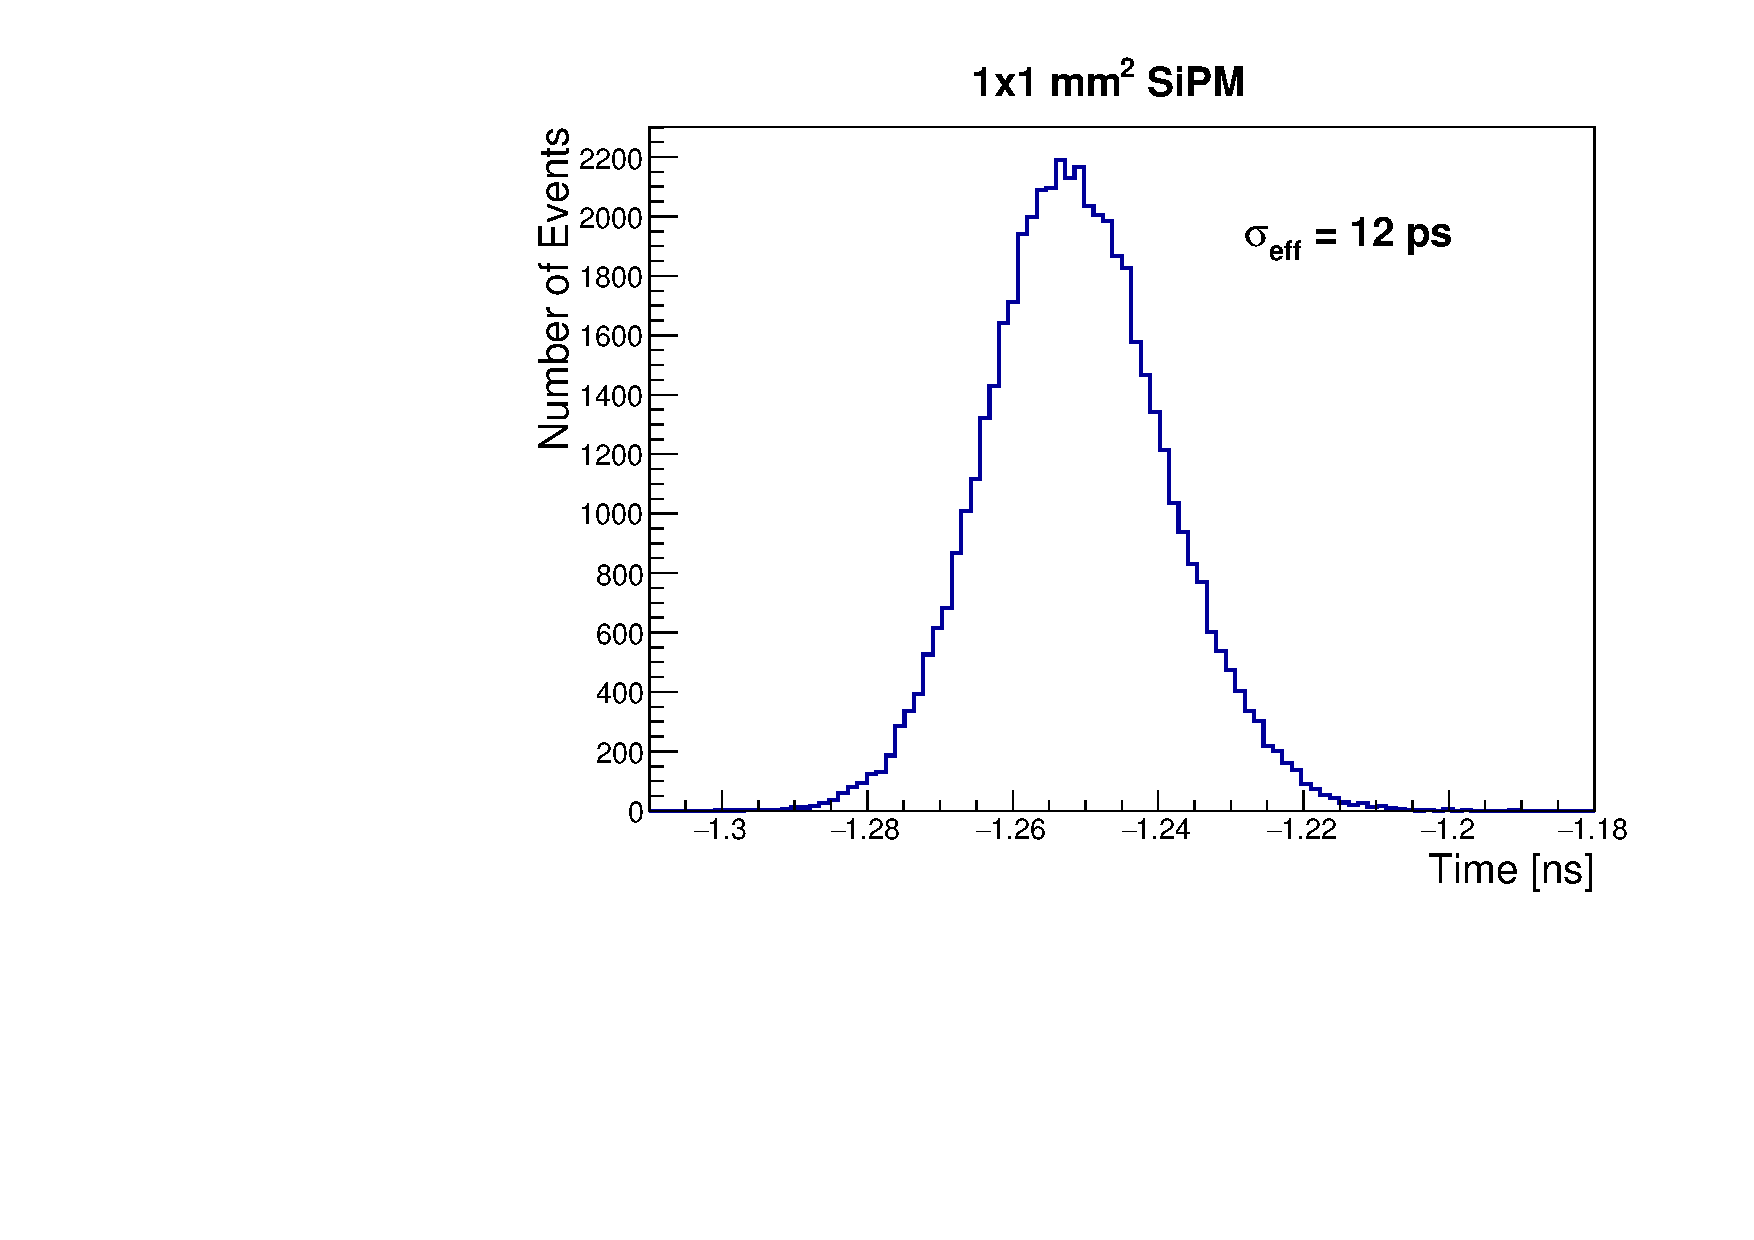
\includegraphics[width=0.49\textwidth]{figures/DeltaT_LargeNPhotons_1x1SiPM.pdf} 
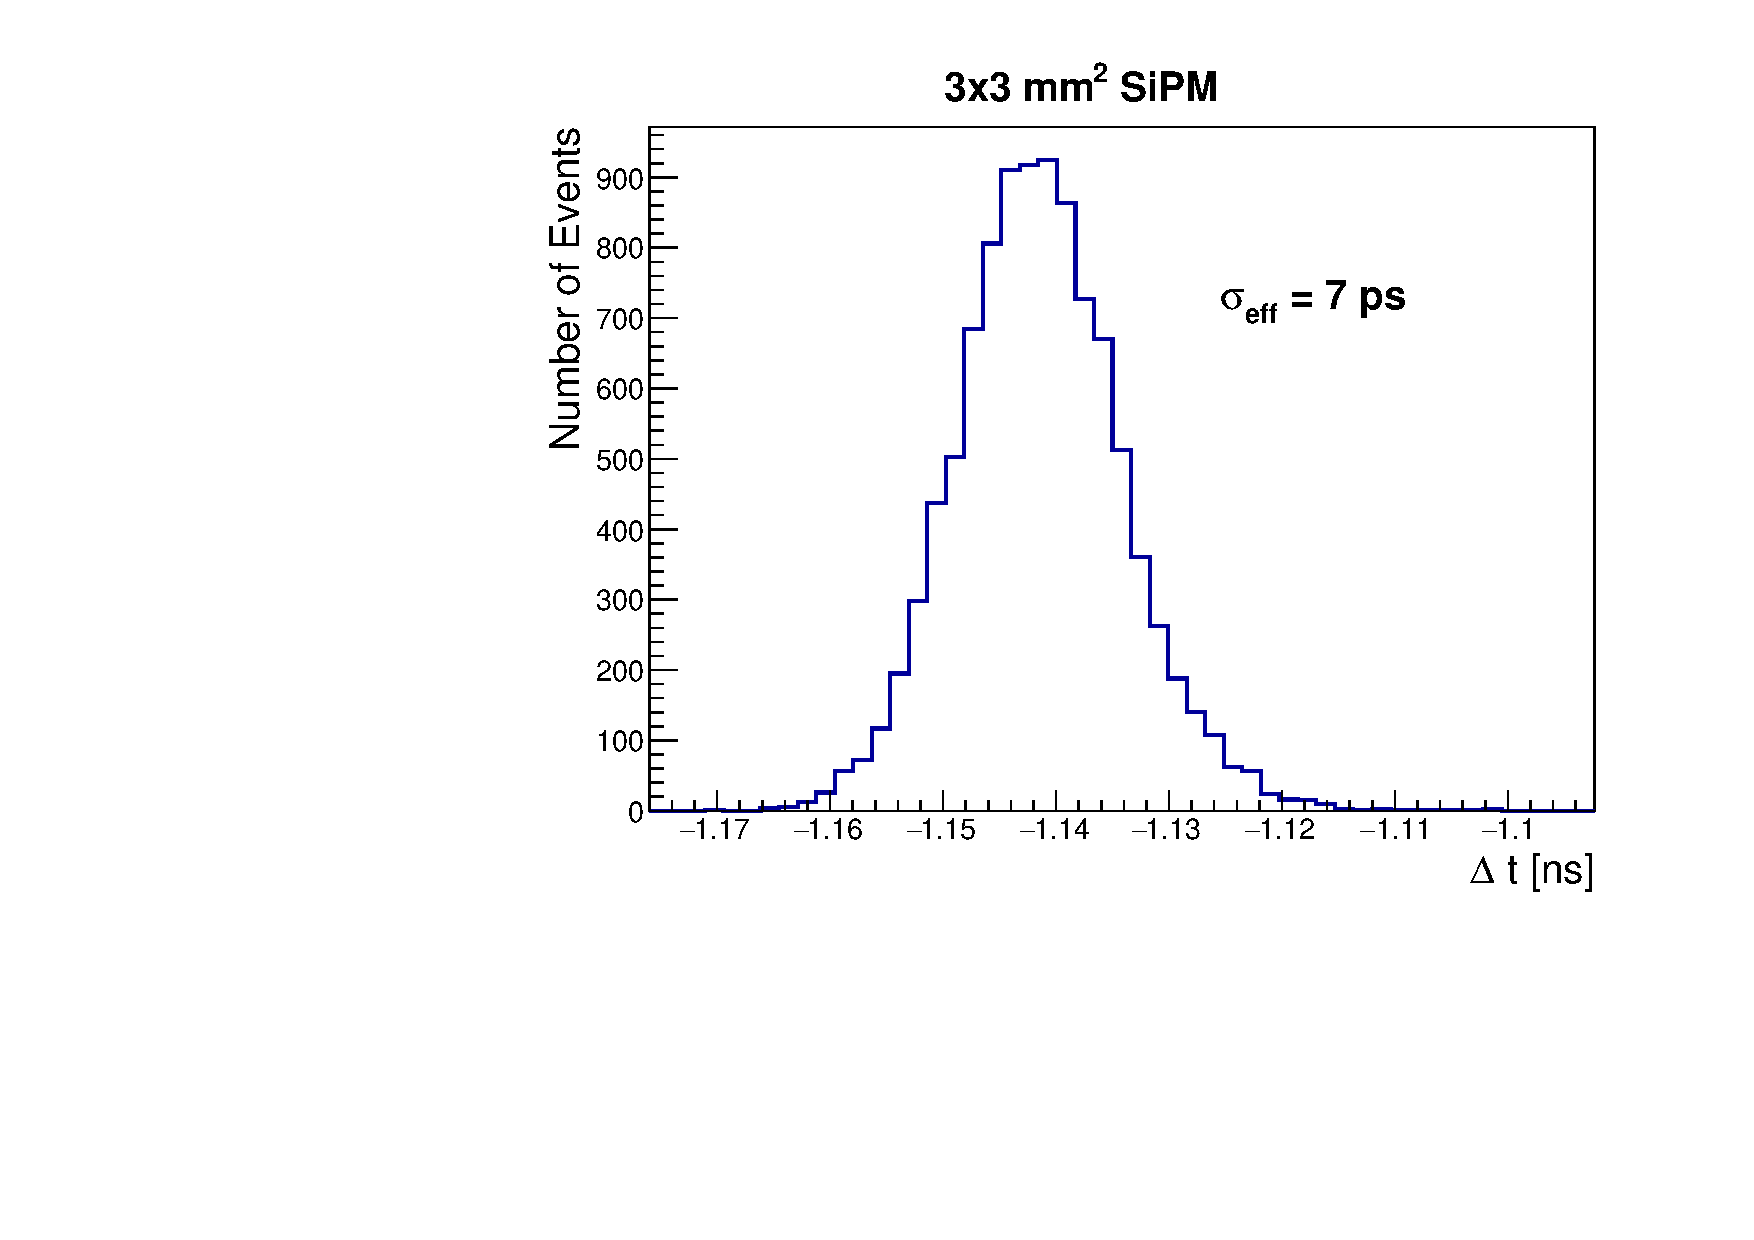
\includegraphics[width=0.49\textwidth]{figures/DeltaT_LargeNPhotons_3x3SiPM.pdf} 
\caption{The SiPM time distribution and resolution measured for laser signals at high laser intensity.} 
\label{fig:LargeLightTimeResolution} 
\end{figure} 

  
%
%
\section{Summary}

We have presented testbeam measurements of the timing performance of a LYSO-based sampling calorimeter
read out via four wavelength shifting fibers optically coupled to silicon photomultipliers (SiPMs).
Time resolutions at the level of $60$~ps is achieved for beam energies above $100$~GeV for individual fibers
and SiPMs. Combining all four fibers yield time resolution measurements of about $42$~ps. Using laser
light injected directly onto SiPMs, we have demonstrated that the impact of the intrinsic time resolution
of the SiPM devices is small and that the calorimeter time resolution is dominated by the impact of the
wavelength shifter. Finally, we have shown that the use of quartz capillaries do not degrade the time resolution
beyond the impact from a reduced signal amplitude. Therefore it is feasible that this
radiation-hard solution using quartz capillaries can achieve the desired $30$~ps time resolution performance if 
additional improvements in light collection efficiency can be achieved.
  
%
%

\section{Acknowledgements} 
Supported by funding from California Institute of Technology High Energy Physics
under Contract DE-SC0011925 with the United States Department of Energy. We
thank the CERN testbeam facilities personnel for excellent beam conditions 
during our testbeam time. We also thank Paolo Meridiani and Francesco Micheli
for their kind assistance on the setup of the DAQ system at the test beam.
%
%
%% If you have bibdatabase file and want bibtex to generate the
%% bibitems, please use
%%
%%  \bibliographystyle{elsarticle-num} 
%%  \bibliography{<your bibdatabase>}

%% else use the following coding to input the bibitems directly in the
%% TeX file.

\bibliography{SiPMTiming}{}
\bibliographystyle{ieeetr} 

\begin{thebibliography}{00}
\bibitem{calor2014} Calorimeters for Precision Timing Measurements in High Energy Physics, A. Bornheim, CALOR2014,doi:10.1088/1742-6596/587/1/012057

\bibitem{lysotiming} On timing properties of LYSO-based calorimeters, D. Anderson, A. Apresyan, A. Bornheim, J. Duarte, C. Pena, A. Ronzhin, M. Spiropulu, J. Trevor, S. Xie, NIM-A, doi:10.1016/j.nima.2015.04.013, 2015

\bibitem{elba2015} Precision Timing Calorimetry for High Energy Physics, A. Bornheim et al, 13th Pisa meeting on Advanced Detectors, Elba 2015, NIM-A doi:10.1016/j.nima.2015.11.129

\bibitem{aashrita}Timing Performance of new Hamamatsu Silicon Photomultipliers, A. Mangu et al, IEEE2014

\bibitem{hama} www.hamamatsu.com



\bibitem{shashlik1} Longevity of the CMS ECAL and Scintillator-Based Options for Electromagnetic Calorimetry at HL-LHC, H. Li, CMS Collaboration, CMS-CR-
2015-127 
\bibitem{shashlik2} A Crystal Shashlik Electromagnetic Calorimeter for Future HEP Experiments, R. Zhu, CALOR2016, these proceedings

\bibitem{capillaries} Studies of Wavelength-Shifting Liquid Filled Quartz Capillaries for Use in a Proposed CMS Calorimeter, B. W. Baumbaugh, R. Ruchti, 
et al, IEEE/NSS2015, Conference Record.




%% \bibitem{label}
%% Text of bibliographic item

%\bibitem{}

\end{thebibliography}

\end{document}
